\chapter{Real-Time Event-Based Optical Flow}\label{sec:ebof}

Following the focus on event cameras, we describe in this second chapter of the thesis how we proposed to solve the ``motion'' part of the subject of the thesis. Beyond allowing for a comprehension of how the ego-platform and external objects are moving in a scene, motion is an essential component for describing the current status of the observed scene, as well as for anticipating its future states. As such, we propose here a real-time optical flow method, which only relies on events from a single camera.

The presented method and the associated results of this chapter were initially published as a journal article in IEEE Transactions on Intelligent Transportation Systems in December 2021~\cite{Brebion2022RealTimeOF}, and were then slightly refined and presented as part of a French national conference (RFIAP) in July 2022~\cite{Brebion2022EstimationDF}. A project page is also available at \url{https://vbrebion.github.io/RTEF/}, and contains the links to the original article, the source code, the dataset, and videos associated to this work.


\section{Introduction}
By estimating the displacement of each pixel in a camera along time, optical flow describes in 2D the motion field of the observed scene. Optical flow is a key enabler for many major applications, such as object detection and tracking~\cite{Braillon2006RealtimeMO}, motion estimation~\cite{Hossen2016ASS}, visual odometry~\cite{Chuanqi2017MonocularVO}, and image segmentation~\cite{Galic2000SpatiotemporalIS}. In the context of intelligent robotics, optical flow constitutes one of the fundamental building bricks of the perception pipeline, especially implied in the detection of moving objects like vulnerable external users.

Optical flow literature is highly abundant for frame-based cameras. However, as discussed in \cref{sec:evtcams:adv_chall:chall:paradigm}, there is no direct translation for frame-based optical flow algorithms to event cameras. The sparse and asynchronous nature of their output constitutes a major paradigm shift. In this chapter, we describe the work conducted over the first year of the thesis, dedicated to this problem. In particular, we describe here our proposition: a novel optimized framework for computing real-time event-based optical flow (\acrshort{ebof}, in short) for both low- and high-resolution event cameras, using a \textit{frame-based} approach. We call our method \acrshort{rtef}, for ``\acrlong{rtef}''.

We first give a formal description of the problem in \cref{sec:ebof:formulation}. Then, in \cref{sec:ebof:sota,sec:ebof:ourorientation}, we review the state of the art of both the frame-based and event-based optical flow methods, and discuss our choice of using a frame-based approach for computing \acrshort{ebof}. Finally, we present our pipeline-based method and evaluate it in \cref{sec:ebof:method,sec:ebof:eval}, before drawing some conclusions in \cref{sec:ebof:conclusion}.


\section{Problem Formulation}\label{sec:ebof:formulation}

The objective of optical flow is to estimate the two-dimensional displacement of intensity patterns~\cite{Fortun2015OpticalFM}. More specifically, in its frame-based formulation, optical flow describes the apparent motion field of pixels between consecutive images, caused by the relative motion between the camera and the elements in the observed scene.

If we note \(I(x, y, t)\) the intensity of a pixel at location \((x, y)\) and at time \(t\), if this pixel moves by \(\Delta x\) and \(\Delta y\) pixels over a period \(\Delta t\) (\(\Delta t\) being the time between two consecutive frames), and if we consider that brightness remains constant over that period, then we have the following equality:

\begin{equation}\label{eq:ebof:formulation_1}
  I(x+\Delta x, y+\Delta y, t+\Delta t) = I(x, y, t)
\end{equation}

By linearizing this equation using Taylor expansion, it can then be shown~\cite{Horn1981DeterminingOF} that:

\begin{equation}\label{eq:ebof:formulation_2}
  I_x u + I_y v + I_t = 0
\end{equation}

where \(I_x\), \(I_y\), and \(I_t\) are respectively the spatial and temporal derivatives (gradients) of the image at coordinates \((x, y)\) and at time \(t\), and where \(u\) and \(v\) are the \(x\) and \(y\) components of the optical flow.

The objective of the optical flow problem is therefore to determine these \(u\) and \(v\) components for every pixel of each pair of consecutive images, in the form of dense motion fields.


\section{Related Work}\label{sec:ebof:sota}

\subsection{Frame-Based Optical Flow}
In \cref{eq:ebof:formulation_2}, the two components \(u\) and \(v\) of the optical flow are unknown, but since only one equation is available, the system is underdetermined (this is the so-called \textit{aperture problem}). To solve this issue, researchers have proposed to add supplementary constraints. In 1981, Horn and Schunck~\cite{Horn1981DeterminingOF} proposed a global \textit{smooth flow} constraint, where flow differences should be minimal for adjacent pixels in the whole image. The same year, Lucas and Kanade~\cite{Lucas1981AnII} proposed a local \textit{constant flow} constraint, where optical flow components should be the same for every pixel of a local neighborhood.

More recent approaches have proposed extensions to these methods. Since the Horn-Schunck and the Lucas-Kanade methods are restricted to small motions, Meinhardt \textit{et al.}~\cite{Meinhardt2013HornSchunckOF} and Bouguet~\cite{Bouguet1999PyramidalIO} proposed pyramidal-based approaches to compute optical flow at multiple scales. To also prevent the oversmoothing of the Horn-Schunck method, Black and Anandan~\cite{Black1996TheRE} and Sun \textit{et al.}~\cite{Sun2013AQA} proposed to add regularization terms, making it more robust.

In the past few years however, a paradigm shift has started appearing, with the transition from geometry-based approaches to learning-based approaches. Neural networks are especially notorious for their capability of learning from data to generalize even in presence of noise and inconsistencies, which is a clear advantage when trying to estimate optical flow on real scenes. Networks like FlowNet~\cite{Dosovitskiy2015FlowNetLO} or UnFlow~\cite{Meister2018UnFlowUL} stood as state of the art over the past few years. However, as proposed by Teed and Deng with RAFT~\cite{Teed2020RAFTRA}, the reintroduction of geometry-based concepts in networks has proven to be an efficient approach.

More recently, unified models able to solve multiple tasks at once have gained popularity, as interactions between these tasks lead to a better understanding of the scene and a better generalization of learned models. The GMFlow network of Xu \textit{et al.}~\cite{Xu2022UnifyingFS} is a perfect example of this trend, as it can compute optical flow, disparity, and depth maps, and as it defines the current state of the art on optical flow.


\subsection[Event-Based Optical Flow]{Event-Based Optical Flow (\acrshort{ebof})}\label{sec:ebof:sota:events}
As noted in \cref{sec:evtcams}, previously listed frame-based methods can not be directly applied to solve the optical flow problem for event cameras. We describe here the various approaches proposed so far in the state of the art, which either try to reformulate the optical flow problem for event-based cameras, or try instead to leverage the frame-based state of the art by converting the event-based optical flow problem into a frame-based problem.

\paragraph{Pure Events} In order to compute event-based optical flow, some authors use the events and all their properties without accumulation into frame-based representations. Such a frameless approach was proposed by Benosman \textit{et al.}~\cite{Benosman2014EventBasedVF}, by using a plane-fitting method on short temporal windows of events to determine their motion in the visual scene. Other works~\cite{Stoffregen2017SimultaneousOF,Gallego2018AUC,Liu2020GloballyOC,Shiba2022SecretsOE,ParedesValls2023TamingCM} proposed contrast maximization schemes as proxies for computing optical flow, by evaluating the sharpness of motion-compensated images of accumulated events. More recently, Paredes-Vallés \textit{et al.}~\cite{ParedesValls2021SelfSupervisedLO,ParedesValls2020UnsupervisedLO} and Cuadrado \textit{et al.}~\cite{Cuadrado2023OpticalFE} proposed to exploit \acrfullpl{snn} for a fully biologically-inspired \acrshort{ebof} estimation.

\paragraph{Reconstructed Frames} Due to the great advances on optical flow estimation with traditional cameras, other authors have proposed to build image-like representations from the events, in order to use them as input for these state-of-the-art methods. Almatrafi \textit{et al.}~\cite{Almatrafi2020DistanceSF} proposed to accumulate events in short temporal windows, to construct a binary image from them, and then to use the distance transform to create stable dense images designed to be used with any frame-based optical flow method. Zhu \textit{et al.}~\cite{Zhu2017EventbasedFT} also proposed to create images of accumulated events, but they instead compute a sparse optical flow by extracting visual features through the use of the Harris corner detector~\cite{Harris1988ACC}, and they track them using an expectation maximization algorithm. An alternative approach was proposed by Nagata \textit{et al.}~\cite{Nagata2021OpticalFE}, as they use a surface matching approach on short time-shifted images of accumulated events (\textit{time surfaces}) to evaluate their displacement.

\paragraph{Learning-Based} Recent works have also adapted proven neural network architectures for a use with images of events; \cite{Zhu2018EVFlowNetSO,Lee2020SpikeFlowNetEO} proposed FlowNet-inspired~\cite{Dosovitskiy2015FlowNetLO} networks for inferring \acrshort{ebof}, while Gehrig \textit{et al.}~\cite{Gehrig2021DenseOF} proposed a RAFT-inspired~\cite{Teed2020RAFTRA} one. Some authors also proposed novel types of networks, designed specifically for the characteristics of event cameras. Paredes-Vallés \textit{et al.}~\cite{ParedesValls2021BackTE} proposed a light and real-time network based on event warping, called FireFlowNet. More recently, Liu \textit{et al.}~\cite{Liu2023TMATM} designed a network able to incorporate the notion of temporal continuity of event data, to compute temporally fine-grained \acrshort{ebof}.

\paragraph{Additional Modalities} Some methods also exploit the capacity of certain neuromorphic sensors to produce more than events, such as frames or inertial measurements. Pan \textit{et al.}~\cite{Pan2020SingleIO} used the flow of events as a deblurring tool for the frames of the DAVIS camera in highly dynamic scenes, allowing for a better optical flow estimation. Rueckauer \textit{et al.}~\cite{Rueckauer2016EvaluationOE} used the IMU integrated in the DAVIS240C camera to determine an exact optical flow estimation for pure rotational movements. Finally, Lee \textit{et al.}~\cite{Lee2021FusionFlowNetEO} extended their FlowNet-inspired network~\cite{Lee2020SpikeFlowNetEO} by adding the grayscale images from the DAVIS camera as a secondary input.


\section{Our Orientation: Densifying Events}\label{sec:ebof:ourorientation}
None of the methods presented in \cref{sec:ebof:sota:events} has considered the issue of computing optical flow with a high-definition event camera. Furthermore, very few of them (\cite{ParedesValls2021BackTE,Liu2020GloballyOC,Rueckauer2016EvaluationOE,Akolkar2020SeeBY}) have been able to achieve real-time compatibility even for low-resolution inputs. In this section, we analyze why both these constraints are difficult to hold, and how we propose to solve them.

First of all, approaches relying on pure events are by definition more complex to develop, as they can not reuse the frame-based state of the art. While they might make the most sense in terms of exploiting the novel event-based paradigm to its full potential, these approaches are especially heavy, slow, and hard to optimize. Furthermore, they have mostly been applied so far to simple scenes with limited motions, and have difficulties scaling to scenes of higher complexity.

Learning-based approaches appear as more promising, as they currently hold state-of-the-art results. However, neural networks always come with a trade-off between the quality of the results and the time it takes for their inference; reaching our objective of real-time performances with a high-resolution input would require sacrificing the quality greatly. Learning-based methods also require a high amount of training data, which is still quite limited to this day for high-resolution sensors. Finally, the quality of the results on never-seen-before scenes is hard to predict, as generalization of the network is not guaranteed, and as it highly relies on the training data, the training procedure, the camera settings, \dots

As such, frame-based approaches are of particular interest to us\footnote{We insist here that we do not aim at fully reconstructing ``real'' images of the scenes like the ones that would be captured by a traditional camera. Instead, we aim at creating pseudo-images, i.e., representations of the event stream as frames which should then be optimized for a use with traditional frame-based optical flow methods.}. Sure, accumulating events to construct pseudo-frames does lead to the loss of the asynchrony property of the event camera, it can lead to losing some precision in the information, and it can reintroduce frame-related problems like motion blur. However, in return, this pseudo-frame construction
\begin{enumerate*}[label=\textbf{(\arabic*)}]
  \item allows for the reuse of frame-based methods which have been developed and optimized over the past decades,
  \item allows for the exploitation of computer architectures to their full potential, especially \acrshortpl{gpu},
  \item can be exploited with traditional geometry-based optical flow approaches, which do not rely on specific training dataset and training procedures, making the quality of results in theory independent of the type of scene observed.
\end{enumerate*}
Furthermore, we underline here that not all properties of the event cameras are lost, and that they are still more interesting than frame-based cameras: the \acrshort{hdr} capacity is still present (so the optical flow should compute similarly during daytime or under low-light), and the event accumulation process can be adjusted on the fly, allowing for a fine control over the level of information that should be kept in a pseudo-frame and the overall responsiveness of the system.


\section{Method}\label{sec:ebof:method}
Following the problem formulation and the reason for the use of a dense representation to reach real-time performances, we detail in this section the novel framework (\acrshort{rtef}) we developed for computing real-time \acrshort{ebof}. In order to optimize computational time and reach real-time performances, we propose to parallelize tasks through the use of a pipeline architecture~\cite{Ramamoorthy1977PipelineA}. An illustration of this framework with example results for each step is available in \cref{fig:ebof:architecture}. The following subsections will detail how each block contributes towards obtaining the real-time \acrshort{ebof}.

\begin{figure}[t]
  \centering
  \begin{tikzpicture}[node distance=4.7cm, scale=0.65, every node/.style={transform shape}]
    % Changing the font
    \fontfamily{cmss}\selectfont

    \draw (0,0) -- (-1,0.5) -- (-1,-0.5) -- cycle;
    \node[draw, align=center, fill=white] (EventCamera) {Event\\camera};

    \node[draw, align=center, label={[name=l1, align=center] below:Events accumulation\\\vphantom{p}}] (Accumulation) [right of=EventCamera, node distance=3.8cm] {\includegraphics[width=0.245\linewidth]{mainmatter/figures/3_optical_flow/architecture/pipeline_edges.png}};
    \node[draw, align=center, label={[name=l2] below:Denoising \& filling}] (Denoising) [right of=Accumulation] {\includegraphics[width=0.25\linewidth]{mainmatter/figures/3_optical_flow/architecture/pipeline_df_edges.png}};
    \node[draw, align=center, label={[name=l3, align=center] below:Negated exponential\\distance transform}] (DistSurf) [right of=Denoising] {\includegraphics[width=0.25\linewidth]{mainmatter/figures/3_optical_flow/architecture/pipeline_ds.png}};
    \node[draw, align=center, label={[name=l4, align=center] below:Real-time frame-based\\optical flow computation}] (RTOF) [right of=DistSurf] {\includegraphics[width=0.25\linewidth]{mainmatter/figures/3_optical_flow/architecture/pipeline_of.png}};
    \node[draw=none] (Out) [right of=RTOF, node distance=3.2cm] {};

    \path[->] (EventCamera) edge[above] node[align=center] {} (Accumulation);
    \path[->] (Accumulation) edge[right] node[align=center] {} (Denoising);
    \path[->] (Denoising) edge[above] node[align=center] {} (DistSurf);
    \path[->] (DistSurf) edge[above] node[align=center] {} (RTOF);
    \path[->] (RTOF) edge[above] node[align=center] {} (Out);

    \node[label={[brown] above:\textbf{\acrshort{cpu}-only}},draw,thick,brown,dotted,fit=(Accumulation)(l1)] {};
    \node[label={[purple] above:\textbf{\acrshort{cpu} and \acrshort{gpu}\vphantom{y}}},draw,thick,purple,dotted,fit=(Denoising)(l2) (DistSurf)(l3) (RTOF)(l4)] {};
  \end{tikzpicture}
  \caption{Our event-based optical flow (\acrshort{ebof}) computation architecture, \acrshort{rtef}, able to run in real-time with low- and high-resolution event cameras. Due to the pipeline architecture, all four blocks are independent parallel processes. Each block depicts the result it produces, for a sample driving sequence.}\label{fig:ebof:architecture}
\end{figure}

\subsection{Accumulation for Edge Images}
As discussed in \cref{sec:ebof:ourorientation}, the very first step needed in our case to ultimately compute optical flow is to accumulate events in the form of a pseudo-image. The first component of our architecture is therefore responsible for receiving and accumulating the events from the camera in short temporal windows, to form ``edge images''. These binary matrices indicate whether each pixel produced at least one event during the accumulation time \(\Delta t\). More formally, if we note \(E(\mathbf{x}, t)\) the content of the pixel at coordinates \(\mathbf{x}\) in the edge image \(E\) produced at time \(t\), then:
\begin{equation}\label{eq:ebof:edge_image}
  \left\{\begin{matrix*}[l]
    E(\mathbf{x}, t) = 1 & \text{if } \exists e=(\mathbf{x}_e, t_e, p_e), \mathbf{x}_e = \mathbf{x}, t \leq t_e < t+\Delta t\\
    E(\mathbf{x}, t) = 0 & \text{otherwise.}
  \end{matrix*}\right.
\end{equation}
By doing so, each edge image depicts a binary representation of the main edges of the objects with relative motion in the visual scene, which can be used as a first stable medium for computing optical flow. For notation simplicity, when the notion of time is not important, we will simply denote the content of a pixel of an edge image as \(E(\mathbf{x})\) in the rest of this chapter.

As can be noted through \cref{eq:ebof:edge_image}, these edge images do not take into account the polarity of the events. As argued by Almatrafi \textit{et al.}~\cite{Almatrafi2020DistanceSF}, and as we have experimented, both positive and negative events represent similarly the edges of the objects in the visual scene. In addition, and as was shown through \cref{fig:evtcams:evts_rel_motion}, polarities are dependent on the orientation of the motion and on their relative color to the background: introducing polarities into the edge images would mean that appearance of objects would change during motion. We want to avoid this phenomenon at all cost if we want to reuse traditional frame-based optical flow methods, which require images to be as stable as possible.

The choice of \(\Delta t\) is also important and linked to the application: taking a \(\Delta t\) too short will lead to edge images with too few events, resulting in an unstable appearance, while taking a \(\Delta t\) too long will fail to capture clearly the movement of the objects by introducing blur.

Compared to other dense formulations from the literature (time surface~\cite{Delbrck2008FramefreeDD,Lagorce2017HOTSAH,Nagata2021OpticalFE}, motion-compensated images~\cite{Gallego2018AUC}, reconstructed images~\cite{Rebecq2021HighSA}), our formulation has the benefit of keeping only the information required for frame-based optical flow estimation. Computationally speaking, this makes this solution extremely efficient, as each packet of events received from the camera only needs to be appended to a buffer. In parallel, a second thread, triggered when the time window has expired, is responsible for collecting all the events from the buffer and creating the edge image, which is then sent for further processing. As such, due to its simplicity, this component runs solely on the \acrshort{cpu}, as it would not benefit from the parallelization capabilities of the \acrshort{gpu}.


\subsection{Denoising and Filling}\label{sec:ebof:denoisingfilling}

Event cameras generate a significant amount of noise, impacting the quality and stability of the edge images, which in return would affect the final optical flow computation if left untreated.

A solution could be to use one of the state-of-the-art denoising solutions of the literature~\cite{Delbrck2008FramefreeDD,Feng2020EventDB} during the accumulation step, that is, before creating the edge image. However, doing so would be computationally expensive, as the sparse and asynchronous nature of the events at that step makes it hard to look for neighbor pixels states. Furthermore, many of these solutions were designed for low-resolution sensors, and translate difficultly to higher definition ones.

To circumvent this issue, we propose in this work a novel, fast yet efficient, method for discarding incorrect events. Our approach relies on applying denoising after the edge image creation. Proposed process is computed in two steps --- denoising and filling --- and is similar to applying morphological erosion and dilatation (morphological opening) on the edge image. In the denoising step, described in \cref{alg:ebof:denoising}, erroneous edge pixels are sought to be eliminated, by removing isolated events. On the contrary, the filling step described in \cref{alg:ebof:filling} aims at filling locations where an edge pixel is missing, but should have been produced by the camera, in order to help to stabilize the edge images. An illustration of both these steps on a real scene is given in \cref{fig:ebof:denoising_filling}.

\begin{algorithm}[ht]
  \caption{Denoising}\label{alg:ebof:denoising}
  \SetKwInOut{Input}{Inputs}
  \Input{An edge image \(E\)\\The denoising threshold \(N_d\)}
  \KwOut{The denoised edge image \(E_d\)}
  \(E_d \gets E\)\;
  \ForEach{pixel index \(\mathbf{x} \in E\)}{
    \If(\tcp*[f]{\(E(\mathbf{x})\) is an edge pixel}){\(E(\mathbf{x}) = 1\)}{
      \(n_d \gets\) count of edge pixels among the 4 direct neighbor pixels of \(\mathbf{x}\) in \(E\)\;
      \If{\(n_d < N_d\)}{
        \(E_d(\mathbf{x}) \gets\) 0 \tcp*{\(E_d(\mathbf{x})\) is not an edge pixel anymore}
      } 
    }
  }
\end{algorithm}

\begin{algorithm}[ht]
  \caption{Filling}\label{alg:ebof:filling}
  \SetKwInOut{Input}{Inputs}
  \Input{A denoised edge image \(E_d\)\\The filling threshold \(N_f\)}
  \KwOut{The denoised and filled edge image \(E_{df}\)}
  \(E_{df} \gets E_d\)\;
  \ForEach{pixel index \(\mathbf{x} \in E_d\)}{
    \If(\tcp*[f]{\(E_d(\mathbf{x})\) is not an edge pixel}){\(E_d(\mathbf{x}) = 0\)}{
      \(n_f \gets\) count of edge pixels among the 4 direct neighbor pixels of \(\mathbf{x}\) in \(E_d\)\;
      \If{\(n_f \geq N_f\)}{
        \(E_{df}(\mathbf{x}) \gets\) 1 \tcp*{\(E_{df}(\mathbf{x})\) becomes an edge pixel}
      }
    }
  }
\end{algorithm}

We underline here the importance of computing denoising and filling separately in this order, to avoid creating inconsistencies. Indeed, if the filling step was processed simultaneously with the denoising, then pixels that would later be discarded as noise could contribute to creating incorrect filling pixels, thus introducing new noise.

Denoising and filling thresholds \(N_d\) and \(N_f\) depend on the event camera configuration, as each camera may give a different noise profile. The aim of the denoising is to discard isolated pixels, that is, pixels with very few neighbors: \(N_d = 1 \text{ or } 2\) appear therefore as the best options. As can be seen in \cref{alg:ebof:denoising}, setting \(N_d = 0\) disables the denoising. Then, the goal of the filling is to slightly stabilize the appearance of the edge images, by adding edge pixels in locations where there are enough neighboring edge pixels to be confident that an edge pixel should have been produced: values of \(N_f = 4 \text{ or } 3\) are therefore the best compromise to add such pixels. As can be seen in \cref{alg:ebof:filling}, setting \(N_f = 5\) disables the filling. A general advice is to select \(N_d < N_f\). A sensitivity analysis on \(N_d\) and \(N_f\) is conducted in \cref{sec:ebof:sensitivity}.

Finally, while this formulation tends to remove small details from the edge images by considering them as noise (as can be seen for instance for the buildings on the right side of the edge images of \cref{fig:ebof:denoising_filling}), it actually helps to obtain more stable images, by extracting the main edges from the scene, and discarding superfluous textures.

\begin{figure}[t]
  \centering
  \begin{subfigure}{0.225\linewidth}
    \centering
    \includegraphics[width=\linewidth]{mainmatter/figures/3_optical_flow/denoising_filling/input.png}
    \caption{}\label{subfig:ebof:denoising_filling:in}
  \end{subfigure}
  \hspace{1mm}
  \begin{subfigure}{0.225\linewidth}
    \centering
    \includegraphics[width=\linewidth]{mainmatter/figures/3_optical_flow/denoising_filling/input_noise_overlaid.png}
    \caption{}\label{subfig:ebof:denoising_filling:noise}
  \end{subfigure}
  \hspace{1mm}
  \begin{subfigure}{0.225\linewidth}
    \centering
    \includegraphics[width=\linewidth]{mainmatter/figures/3_optical_flow/denoising_filling/denoised_filling_overlaid.png}
    \caption{}\label{subfig:ebof:denoising_filling:fill}
  \end{subfigure}
  \hspace{1mm}
  \begin{subfigure}{0.225\linewidth}
    \centering
    \includegraphics[width=\linewidth]{mainmatter/figures/3_optical_flow/denoising_filling/output.png}
    \caption{}\label{subfig:ebof:denoising_filling:out}
  \end{subfigure}
  \caption{Steps of the denoising and filling process, for a noisy edge image. A zoomed view of the streetlamp (squared in yellow) is also provided for better visibility. (\subref{subfig:ebof:denoising_filling:in}) The original noisy edge image. (\subref{subfig:ebof:denoising_filling:noise}) The same image with edge pixels identified as noise in red (\(N_d = 2\)). (\subref{subfig:ebof:denoising_filling:fill}) The denoised edge image with the newly added pixels for the filling in green (\(N_f = 3\)). (\subref{subfig:ebof:denoising_filling:out}) The final denoised and filled edge image.}\label{fig:ebof:denoising_filling}
\end{figure}

Another advantage of this formulation lies in its simple and parallelizable formulation, as the computation for each pixel is independent of the one of its neighbors. Therefore, we implemented it on the \acrshort{gpu}, to exploit its capabilities, and to relieve the \acrshort{cpu} so that it can undertake other complex tasks.

\subsection{The Negated Exponential Distance Surface}\label{sec:ebof:inv_exp_dist_surf}
Even after denoising and filling, the edge images are only binary matrices. As such, they can hardly be used for computing optical flow with traditional frame-based algorithms: as shown in \cref{eq:ebof:formulation_2}, these methods require image gradients, which would be discontinuous for our binary edge images. In order to make them viable for frame-based optical flow computation, densifying them through the use of the distance transform, as proposed by Almatrafi \textit{et al.}~\cite{Almatrafi2020DistanceSF}, is an interesting baseline for introducing smooth variations in the images, and therefore having smooth gradients.

In their approach, they consider a set of edge pixels \(\Phi\), which is defined in our case after denoising and filling as:
\begin{equation}
  \Phi \doteq \{\mathbf{x}_i \mid E_{df}(\mathbf{x}_i) = 1\}
\end{equation}
Then, they compute a distance surface \(D\) (which is of the same size as the edge image), by giving to each pixel \(\mathbf{x}\) of \(D\) its distance to the closest edge pixel in \(\Phi\). Formally, it can be written as follows:
\begin{equation}
  D(\mathbf{x}) \doteq \min_{\mathbf{x}_i \in \Phi} d(\mathbf{x}, \mathbf{x}_i)
\end{equation}
where \(d\) is the L\textsuperscript{2} distance function:
\begin{equation}
  d(\mathbf{x}_1, \mathbf{x}_2) \doteq \sqrt{(\mathbf{x}_1 - \mathbf{x}_2)(\mathbf{x}_1 - \mathbf{x}_2)^T}
\end{equation}
In order to obtain an actual 8-bit image, a final normalization is applied to contain the values of the distance surface as integers between 0 and 255:
\begin{equation}\label{eq:ebof:dist_surf_norm}
  D_\text{normalized}(\mathbf{x}) \doteq \round*{255 \times \frac{D(\mathbf{x})}{\max(D)}}
\end{equation}

\begin{figure}[t]
  \centering
  \setlength{\tabcolsep}{1mm}
  \begin{tabular}{@{}ccccc@{}}
    & \multirow{2}{*}{Edge image} & Distance surface & Our negated exp. & \multirow{2}{*}{Gaussian blur} \\
    & & {\small(Almatrafi \textit{et al.}~\cite{Almatrafi2020DistanceSF})} & distance surface & \\
    \raisebox{1.2cm}[0pt][0pt]{\rotatebox[origin=c]{90}{Missing pxls}} &
    \includegraphics[width=0.22\linewidth]{mainmatter/figures/3_optical_flow/distance_surface/missing_events.png} &
    \includegraphics[width=0.22\linewidth]{mainmatter/figures/3_optical_flow/distance_surface/orig_ds_missing_events.png} &
    \includegraphics[width=0.22\linewidth]{mainmatter/figures/3_optical_flow/distance_surface/exp_ds_missing_events.png} &
    \includegraphics[width=0.22\linewidth]{mainmatter/figures/3_optical_flow/distance_surface/gauss_missing_events.png} \\
    \raisebox{1.2cm}[0pt][0pt]{\rotatebox[origin=c]{90}{Noise}} &
    \includegraphics[width=0.22\linewidth]{mainmatter/figures/3_optical_flow/distance_surface/noise_red_circle.png} &
    \includegraphics[width=0.22\linewidth]{mainmatter/figures/3_optical_flow/distance_surface/orig_ds_noise.png} &
    \includegraphics[width=0.22\linewidth]{mainmatter/figures/3_optical_flow/distance_surface/exp_ds_noise.png} &
    \includegraphics[width=0.22\linewidth]{mainmatter/figures/3_optical_flow/distance_surface/gauss_noise.png} \\
    \raisebox{1.2cm}[0pt][0pt]{\rotatebox[origin=c]{90}{Position}} &
    \includegraphics[width=0.22\linewidth]{mainmatter/figures/3_optical_flow/distance_surface/moved_bottom_right.png} &
    \includegraphics[width=0.22\linewidth]{mainmatter/figures/3_optical_flow/distance_surface/orig_ds_moved_bottom_right.png} &
    \includegraphics[width=0.22\linewidth]{mainmatter/figures/3_optical_flow/distance_surface/exp_ds_moved_bottom_right.png} &
    \includegraphics[width=0.22\linewidth]{mainmatter/figures/3_optical_flow/distance_surface/gauss_moved_bottom_right.png} \\
    \raisebox{1.2cm}[0pt][0pt]{\rotatebox[origin=c]{90}{Real scene}} &
    \includegraphics[width=0.22\linewidth]{mainmatter/figures/3_optical_flow/distance_surface/indoor_flying.png} &
    \includegraphics[width=0.22\linewidth]{mainmatter/figures/3_optical_flow/distance_surface/indoor_flying_orig_ds.png} &
    \includegraphics[width=0.22\linewidth]{mainmatter/figures/3_optical_flow/distance_surface/indoor_flying_exp_ds.png} &
    \includegraphics[width=0.22\linewidth]{mainmatter/figures/3_optical_flow/distance_surface/indoor_flying_gauss.png} \\
  \end{tabular}
  \caption{Comparison between the original distance surface, proposed negated exponential distance one (with \(\alpha=8\) for a good visibility), and a simple Gaussian blur (with \(\sigma=3\text{px}\)). From top to bottom: a simulated square with 50\% of its pixels randomly removed; the same square with a single pixel of noise added (circled in red); the same square in the bottom right of the image; and an indoor flying scene from the MVSEC dataset~\cite{Zhu2018TheMS}.}\label{fig:ebof:distance_surfaces}
\end{figure}

However, this approach has the main drawback of needing a near-perfect denoising, as a single noisy event can disrupt the appearance of the whole distance surface, as shown in the second row of \cref{fig:ebof:distance_surfaces}. The computed distances do not have an upper bound, meaning that the area of influence of each edge pixel can be infinite, and depends on the presence of other close neighbors. In addition, as shown in \cref{eq:ebof:dist_surf_norm}, the image representation of the distance surface depends on its maximum value, and the appearance of objects can therefore vary greatly based on their position. An example of this behavior is shown in the third row of \cref{fig:ebof:distance_surfaces}: the inside part of the square appears darker when it is in the bottom right of the image, due to the maximum distance increasing. An answer to these problems could be to limit the computed distances to a maximal value, restricting the influence of an edge pixel to a fixed neighborhood. This solution, however, would introduce a non-smooth transition in the distance transform function. It can become an issue for the gradient computation on distance surfaces, often used as part of the optical flow estimation.

Another issue of the approach of Almatrafi \textit{et al.} also appears when distinct objects come close to each other: their edges tend to merge together in the resulting distance surface, making the individual objects indistinguishable, such as in the last row of \cref{fig:ebof:distance_surfaces}. This phenomenon can lead to incorrect optical flow results, especially when a block-matching or image warping formulation is employed, due to the lack of texture on the produced image. Giving more emphasis to the pixels directly surrounding the edge pixels would help to create distance surfaces with more prominent object edges, limiting this merging issue. A solution could be to employ a function with a logarithmic shape.

\begin{figure}[t]
  \centering
  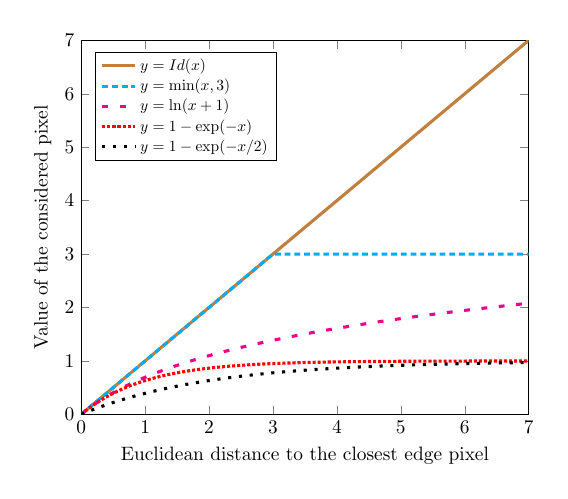
\begin{tikzpicture}[scale=0.7, every node/.style={transform shape}]
    \begin{axis}[width=.8\linewidth, xmin=0, xmax=7, ymin=0, ymax=7, xlabel={Euclidean distance to the closest edge pixel}, ylabel={Value of the considered pixel}, legend style={nodes={scale=0.8, transform shape}}, legend pos=north west, legend cell align=left, samples=200]
      \addplot[brown, domain=0:7, ultra thick] {x};
      \addplot[cyan, domain=0:7, densely dashed, ultra thick] {min(x, 3)};
      \addplot[magenta, domain=0:7, loosely dashed, ultra thick] {ln(x+1)};
      \addplot[red, domain=0:7, densely dotted, ultra thick] {1-exp(-x)};
      \addplot[domain=0:7, loosely dotted, ultra thick] {1-exp(-x/2)};
      \addlegendentry{\(y = \func{Id}(x)\)}
      \addlegendentry{\(y = \min(x, 3)\)}
      \addlegendentry{\(y = \ln(x+1)\)}
      \addlegendentry{\(y = 1-\exp(-x)\)}
      \addlegendentry{\(y = 1-\exp(-x/2)\)}
    \end{axis}
  \end{tikzpicture}
\caption{Values of the distance transform as a function of the distance to the closest edge pixel. In the order of the legend, the curves represent the original distance transform, the same with an upper bound set to 3px, the natural logarithm version, and our negated exponential formulation, with \(\alpha \) set to 1 and 2 respectively.}\label{fig:ebof:distance_surface_plot}
\end{figure}

To solve jointly both these issues, we propose in this work to replace the distance surface \(D\) with a novel negated exponential distance surface \(D_\text{exp}\), formulated as follows:
\begin{equation}
  D_\text{exp}(\mathbf{x}) \doteq \min_{\mathbf{x}_i \in \Phi} d_\text{exp}(\mathbf{x}, \mathbf{x}_i)
\end{equation}
where \(d_\text{exp}\) is a negated exponential distance function:
\begin{equation}\label{eq:ebof:negated_exp_dist}
  d_\text{exp}(\mathbf{x}_1, \mathbf{x}_2) \doteq 1-\exp\left({-\frac{d(\mathbf{x}_1, \mathbf{x}_2)}{\alpha}}\right)
\end{equation}
where \(\alpha \) is a spreading parameter. \Cref{fig:ebof:distance_surface_plot} compares the aforementioned functions over the distance to the closest edge pixel. As can be seen through the plot, the main advantage of our negated exponential formulation is that, while close to a logarithmic formulation, each edge pixel also has a restricted influence area, after which the values saturate to a value of 1. Therefore, the normalized 8-bit image version can then be re-written as:
\begin{equation}
  D_\text{exp\_normalized}(\mathbf{x}) \doteq \round*{255 \times D_\text{exp}(\mathbf{x})}
\end{equation}
where the dependence on the maximum distance is removed.

The spreading parameter \(\alpha \) can be used to determine the size of the neighborhood influenced by each edge pixel. This parameter conditions the appearance of the distance surface, and regulates the remaining imperfections of the edge images. A low value for \(\alpha \) restricts the area of influence of each edge pixel to only its close neighbors. It limits the influence of the noise on its appearance, but makes the distance surface less stable and more prone to variations. On the contrary, selecting a higher value for \(\alpha \) has the opposite effect: variations of the appearance of the various objects in the scene are well compensated, but noisy events have a more important effect.

In addition, \(\alpha\) can be rewritten from \cref{eq:ebof:negated_exp_dist} as a function of the wanted distance of saturation for \(d\), which we will name here \(d_\text{sat}\) (we remove the function parameters for more simplicity in the notations):
\begin{equation}\label{eq:ebof:alpha_fct_dsat_eps}
  \alpha = -\frac{d_\text{sat}}{\ln(\varepsilon)}
\end{equation}
with
\begin{equation}
  \varepsilon \doteq 1-d_\text{exp}
\end{equation}
where by definition \(\varepsilon > 0\). \(\varepsilon \) is formulated so as to represent the gap between \(d_\text{exp}\) and the saturation value of \(1\). Saturation is therefore reached when this gap \(\varepsilon \) is as small as possible, i.e., \(\varepsilon \to 0\). Since we work in the discrete 8-bit domain, saturation is reached when \(\varepsilon < 1/255\). Integrating this value in \cref{eq:ebof:alpha_fct_dsat_eps} results in the final formulation of \(\alpha \) as a function of \(d_\text{sat}\):
\begin{equation}
  \alpha = -\frac{d_\text{sat}}{\ln(1/255)} \approx \frac{d_\text{sat}}{5.541}.
\end{equation}
The sensitivity of \(d_\text{sat}\) is studied in the analysis \cref{sec:ebof:sensitivity}.

The interest of our negated exponential distance surface formulation is illustrated in \cref{fig:ebof:distance_surfaces} as a side-by-side visual comparison with the original distance surface. As expected, our negated exponential formulation compensates the missing pixels similarly to the original distance surface, while limiting the impact of noisy edge pixels. As seen in the third row, the appearance of objects also remains the same independently of their position, due to the removal of the dependence on the maximum distance in the image normalization process. Finally, this formulation displays more distinct edges and keeps objects texture, especially visible in the real complex scene represented in the last row (note how the board and the barrel keep a clear appearance using negated exponential formulation, while they are hardly distinguishable with the original distance surface).

In addition, while at first glance a simple Gaussian blur could be considered to have similar effects to our formulation for a lower computational cost, we showcase in \cref{fig:ebof:distance_surfaces} that this is not really the case. Missing pixels are much less compensated as seen in the first row, while areas with more edge pixels appear darker in the last row. Both these phenomenons are due to the use of a kernel for blurring the image: the more edge pixels fall into the kernel centered around a given pixel, the higher the value of this pixel will be, meaning that the value of a pixel depends on its close neighbors. This is something we want to avoid at all cost, since we want to make objects as similar-looking as possible through time for a good computation of optical flow.

Regarding the implementation of the distance transform, we employed the fast solution described by Coeurjolly \textit{et al.}~\cite{Coeurjolly2007GomtrieDE}. The choice of this method was especially motivated by its optimized formulation, allowing for large parallelization, and by the little amount of modifications required to incorporate our negated exponential formulation. This block of our pipeline was therefore also implemented on \acrshort{gpu}, to exploit its parallelization capabilities.

\subsection{Frame-Based Optical Flow}\label{sec:ebof:of}
The final block of our architecture is the computation of the optical flow itself. Since the previous steps led to dense image-like structures from the flow of events, any state-of-the-art frame-based optical flow method could be used here.

As part of this work, we selected the ``flow filter'' approach of Adarve and Mahony~\cite{Adarve2016AFF}. Their method is based on an update-prediction architecture, similar to the one of Black~\cite{Black1992RobustIO}, which predicts optical flow using an image warping process, and temporally propagates the optical flow estimations using an incremental framework. Multiple update-prediction loops are stacked as a pyramidal structure, enabling the capture of both large and fine displacements in the images. Their method was designed for a fast and accurate estimation of the optical flow field, and is implemented on \acrshort{gpu}.

The choice of this method as our optical flow computation solution was mainly guided by their use of a predictive filter-based formulation, which, beyond enabling real-time compatibility on \acrshort{gpu}, allows for a temporal smoothing of the flow. This property brings stability and robustness to the overall optical flow thanks to its memory effect, which is beneficial given the sometimes unstable nature of events.

Finally, while this method returns a dense optical flow covering the whole surface of the image, we restrict it to the edge pixels of the denoised and filled edge image. Indeed, by nature, events encode sparse information, detailing the pixels for which a change in luminosity was observed. The densification produced by the use of the negated exponential distance transform differs from an inference of missing data: it is only intended for creating texture and smooth transitions, which are necessary to determine the optical flow.


\section{Evaluation}\label{sec:ebof:eval}

\subsection{Datasets}

As part of the evaluation of the proposed methods, five datasets are going to be used in the following subsections. The first one is the low-resolution MVSEC dataset~\cite{Zhu2018EVFlowNetSO,Zhu2018TheMS}, which was the first event vision dataset with real data that included a ground truth optical flow. However, as noted in \cref{sec:evtcams:datasets}, the MVSEC dataset suffers from several limitations (lack of physical synchronization, approximate calibration, \dots). While it remains an interesting baseline, its use starts to decline now that more recent datasets have been published. As such, we will also evaluate our method on the mid-resolution DSEC dataset~\cite{Gehrig2021DSECAS}, which constitutes a more stable benchmark. Both will serve as the basis for comparison with other state-of-the-art methods. For high-definition data, three complementary datasets are used: the 1 Megapixel Automotive Detection Dataset~\cite{Perot2020LearningTD}, for a deep evaluation on daily driving sequences; a 20-minute-long driving sequence recorded by Prophesee, for visual comparison with the current frame-based state of the art; and a novel high-speed high-definition event-based indoor dataset we recorded as part of this thesis, to demonstrate the accuracy of \acrshort{rtef} even under large motions. A summary of these datasets is given in \cref{tab:ebof:datasets_comp}.

\begin{table}[ht]
  \centering
  \resizebox{\linewidth}{!}{
    \begin{tabular}{@{}lccccc@{}}
      \toprule
      & Resolution & Scenes & Ground truth? & Frames? & Conditions \\
      \midrule
      MVSEC & \(346\times240\) (low) & Indoor \& Vehicular & Semi-dense & Yes & Day, night \\
      DSEC & \(640\times480\) (mid) & Vehicular & Semi-dense & Yes & Day, night \\
      1 Megapixel Automotive Detection & \(1280\times720\) (\acrshort{hd}) & Vehicular & No & No & Day, varying lighting and weather \\
      20-minute-long driving sequence & \(1280\times720\) (\acrshort{hd}) & Vehicular & No & Yes & Day, single long sequence \\
      Our high-speed event dataset & \(1280\times720\) (\acrshort{hd}) & Indoor & No & No & Very fast and erratic motions \\
      \bottomrule
    \end{tabular}
  }
  \caption{Comparison of the event-based datasets used for the evaluation of our optical flow method \acrshort{rtef}.}\label{tab:ebof:datasets_comp}
\end{table}

\subsection{Setup}\label{sec:ebof:setup}
The implementation of our method was made using ROS Noetic, in \CC{}11 and CUDA 12.2, combined with the use of the OpenCV 4.2 library. Both the implementation and the evaluation phases were conducted on an HP ZBook 17 G6 laptop, with an Intel i9-9880H CPU, an NVIDIA Quadro RTX 5000 GPU, 64 GB of RAM, and using Ubuntu 20.04.

Regarding the parameters, three configurations were used, respectively for low-, mid-, and high-resolution input data.

For the low-resolution data (\(346\times260\)) of the MVSEC dataset~\cite{Zhu2018EVFlowNetSO,Zhu2018TheMS}, we were restricted to use a temporal window of size \(\Delta t = 1\text{ frame}\)\footnote{In MVSEC, \(\Delta t = 1\text{ frame} \simeq 32\text{ms}\) for ``Indoor flying'' sequences, \(\simeq 22\text{ms}\) for ``Outdoor day'' sequences, and \(\simeq 97\text{ms}\) for ``Outdoor night'' sequences.} for a fair comparison with the other state-of-the-art methods using this time window~\cite{Zhu2019UnsupervisedEL,Zhu2018EVFlowNetSO,ParedesValls2021SelfSupervisedLO,Gehrig2021DenseOF,ParedesValls2021BackTE,Lee2020SpikeFlowNetEO,Akolkar2020SeeBY,Stoffregen2020ReducingTS}. For the denoising and filling, we set \(N_d = 1\) and \(N_f = 4\), due to the high noise in these recordings. The negated exponential distance transform was configured with \(\alpha = 1.08\) (so that \(d_\text{sat} = 6\text{px}\), see \cref{eq:ebof:alpha_fct_dsat_eps}). Finally, the ``flow filter'' method of Adarve and Mahony~\cite{Adarve2016AFF} was configured with 3 pyramidal layers, with their regularization weights set respectively to \(50.0\), \(250.0\), and \(500.0\), and with \(50\), \(25\), and \(5\) smooth iterations per layer.

For the mid-resolution data (\(640\times480\)) of the DSEC dataset~\cite{Gehrig2021DSECAS}, we used a temporal window of size \(\Delta t = 20\text{ms}\), instead of the intended \(\Delta t = 100\text{ms}\) one (more discussion on that topic is given in \cref{sec:ebof:eval_dsec}). No denoising nor filling was used on this dataset (\(N_d = 0\), \(N_f = 5\)), due to the low amount of noise in these recordings. Similarly to the low-resolution data, \(\alpha\) was set to a value of 1.08 (\(d_\text{sat} = 6\text{px}\)), and the ``flow filter'' method was configured with 3 layers, with their regularization weights set respectively to \(5.0\), \(150.0\), and \(200.0\), and with \(200\), \(150\), and \(7\) smooth iterations per layer.

For the high-resolution data (\(1280\times720\)), finally, a temporal window \(\Delta t = 15\text{ms}\) was used, to better capture the movements. \(N_d = 2\) and \(N_f = 3\) were empirically chosen, as the best compromise between removing noise and keeping the main edges. \(\alpha=1.08\) (\(d_\text{sat} = 6\text{px}\)) also proved to be the more adequate, allowing to keep the scene details, while compensating potential imperfections. The ``flow filter'' method was configured with 3 layers, with regularization weights all set to \(500.0\), and with \(20\) smooth iterations per layer.

Finally, in the \acrshort{ebof} illustrations and videos in the following subsections, the pixels where no event was received are colored in medium gray.

\subsection{Evaluation Metrics}
In order to evaluate the quality of our optical flow results, three metrics are used as part of this chapter.

The first two ones, the percentage of outliers and the \acrfull{aee}, are traditional optical flow metrics, used for instance in the KITTI benchmark~\cite{Geiger2012AreWR}. The percentage of outliers reports the number of pixels for which the error is above 3px and 5\% of the magnitude of the flow vector. The \acrshort{aee} is a raw error measurement on both orientation and magnitude of the flow, computed as following:
\begin{equation}\label{eq:ebof:aee}
  \text{AEE} = \frac{1}{N}\sum_{i=1}^{N}|f_i-\hat{f_i}|
\end{equation}
where \(N\) is the total number of flow vectors, \(f_i\) the \(i\)\textsuperscript{th} estimated flow vector, and \(\hat{f_i}\) its ground truth equivalent.

However, still as of the writing of this thesis, no complex high-resolution event-based dataset with a ground truth for optical flow exists. In order to still leverage high-resolution datasets, for instance Prophesee's 1 Megapixel Automotive Detection dataset~\cite{Perot2020LearningTD}, and to provide a quantitative evaluation of our \acrshort{ebof} results, we adopt the \acrfull{fwl} metric proposed by Stoffregen \textit{et al.}~\cite{Stoffregen2020ReducingTS}. The principle is to compensate the motion of each raw event (considering its polarity and timestamp) through its computed optical flow, in order to accumulate them in an image of compensated events at a reference time \(t\). If the optical flow is accurate, compensated events superimpose in the same pixel position, producing sharp edges. The \acrshort{fwl} then evaluates the sharpness of the produced image, compared to the one where events are not compensated:
\begin{equation}
  \text{FWL} = \frac{\sigma^2(I_\text{comp})}{\sigma^2(I_\text{uncomp})}
\end{equation}
where \(\sigma^2\) is the image variance function, \(I_\text{comp}\) the flow-compensated image of events, and \(I_\text{uncomp}\) the original uncompensated image. By doing so, a final \acrshort{fwl} value greater than \(1\) is sought to be obtained, as it indicates that the computed flow is better than the ``zero flow'' (uncompensated) reference, as the compensated image is more sharp.

While the \acrshort{fwl} metric allows for comparison on datasets without a ground truth, it suffers from several issues. One such issue is the ``event collapse'' highlighted by Shiba \textit{et al.}~\cite{Shiba2022SecretsOE}: high \acrshort{fwl} scores are obtained if the motion of all events is compensated such that they fall in the same pixel, resulting in images with a maximal sharpness. While such an issue was not observed in our case, results presented with this metric should therefore still be taken with a grain of salt.

\subsection{Ablation Studies}
To show the validity of our contributions, we also conducted evaluations with ablations or distance surface alternatives:
\begin{itemize}
  \item RTEF\textsubscript{NDF}, the full proposition without denoising and filling;
  \item RTEF\textsubscript{DS\_L}, with the linear distance transform, \(y = \func{Id}(x)\);
  \item RTEF\textsubscript{DS\_LB}, with the upper-bound distance transform (set to 6px, equal to the used \(d_\text{sat}\) value with proposed negated exponential formulation), \(y = \min(x, 6)\);
  \item RTEF\textsubscript{DS\_Log}, with the logarithmic distance transform, \(y = \log_e(x+1)\).
\end{itemize}
As a reminder, \cref{fig:ebof:distance_surface_plot} illustrates the shape of these variants.


\subsection{Evaluation on the MVSEC Dataset}\label{sec:ebof:eval_mvsec}
We first evaluate our \acrshort{ebof} method on the low-resolution (\(346\times260\)) MVSEC dataset proposed by Zhu \textit{et al.}~\cite{Zhu2018EVFlowNetSO,Zhu2018TheMS}. Despite several shortcomings highlighted by its authors --- namely, errors created by moving objects, an approximate synchronization, an approximate calibration, and the use of default biases for the event camera --- this dataset remains the main reference for evaluating \acrshort{ebof} results on complex real-life sequences. Therefore, we present in \cref{tab:ebof:mvsec_results} our error measurements on this dataset, compared to other reference methods from the literature (both non real-time and real-time capable). We also compare them to a ``zero flow'' reference, i.e., error measurements when the estimated optical flow is set to a null vector field. Note that, similarly to other authors such as \cite{Zhu2018EVFlowNetSO, Stoffregen2020ReducingTS}, for \verb|outdoor| sequences, we ignored the pixels where the hood of the car is visible, as the ground truth values for these pixels are incorrect in the MVSEC dataset.

\begin{table}[ht]
  \centering
  \resizebox{\linewidth}{!}{
    \begin{tabular}{@{}l cc cc cc cc cc cc cc cc@{}}
      \toprule
      & \multicolumn{2}{c}{\Verb|indoor_flying_1|} & \multicolumn{2}{c}{\Verb|indoor_flying_2|} & \multicolumn{2}{c}{\Verb|indoor_flying_3|} & \multicolumn{2}{c}{\Verb|outdoor_day_1|} & \multicolumn{2}{c}{\Verb|outdoor_day_2|} & \multicolumn{2}{c}{\Verb|outdoor_night_1|} & \multicolumn{2}{c}{\Verb|outdoor_night_2|} & \multicolumn{2}{c}{\Verb|outdoor_night_3|} \\ \cmidrule(lr){2-3} \cmidrule(lr){4-5} \cmidrule(lr){6-7} \cmidrule(lr){8-9} \cmidrule(lr){10-11} \cmidrule(lr){12-13} \cmidrule(lr){14-15} \cmidrule(lr){16-17}
      & \acrshort{aee}~\(\downarrow{}\) & \% outl.~\(\downarrow{}\) & \acrshort{aee}~\(\downarrow{}\) & \% outl.~\(\downarrow{}\) & \acrshort{aee}~\(\downarrow{}\) & \% outl.~\(\downarrow{}\) & \acrshort{aee}~\(\downarrow{}\) & \% outl.~\(\downarrow{}\) & \acrshort{aee}~\(\downarrow{}\) & \% outl.~\(\downarrow{}\) & \acrshort{aee}~\(\downarrow{}\) & \% outl.~\(\downarrow{}\) & \acrshort{aee}~\(\downarrow{}\) & \% outl.~\(\downarrow{}\) & \acrshort{aee}~\(\downarrow{}\) & \% outl.~\(\downarrow{}\) \\
      \midrule
      \midrule
      Zero flow & 1.71 & 8.9 & 3.03 & 40.2 & 2.53 & 29.1 & 1.46 & 5.1 & 1.70 & 13.0 & 5.41 & 63.8 & 6.62 & 73.7 & 7.20 & 77.1 \\
      \midrule
      \midrule
      \multicolumn{17}{c}{\textbf{Non Real-Time}} \\
      EV-FlowNet\textsubscript{MVSEC}\textsuperscript{*}~\cite{Zhu2018EVFlowNetSO} & 0.85 & 0.9 & 1.29 & 7.5 & 1.13 & 5.3 & 0.56 & 0.4 & - & - & \textbf{1.90} & \textbf{18.6} & \textbf{2.26} & \textbf{21.9} & \textbf{2.13} & \textbf{20.4} \\
      Zhu \textit{et al.}~\cite{Zhu2019UnsupervisedEL} & 0.58 & \textbf{0.0} & 1.02 & 4.0 & 0.87 & 3.0 & 0.32 & \textbf{0.0} & - & - & - & - & - & - & - & - \\
      EV-FlowNet\textsubscript{HQF}~\cite{Stoffregen2020ReducingTS} & 0.56 & - & 0.66 & - & 0.59 & - & 0.68 & - & \textbf{0.82} & - & - & - & - & - & - & - \\
      Spike-FlowNet~\cite{Lee2020SpikeFlowNetEO} & 0.84 & - & 1.28 & - & 0.87 & - & 0.49 & - & - & - & - & - & - & - & - & - \\
      Spiking EV-FlowNet~\cite{ParedesValls2021SelfSupervisedLO} & 0.60 & 0.5 & 1.17 & 8.1 & 0.93 & 5.6 & 0.47 & 0.2 & - & - & - & - & - & - & - & - \\
      E-RAFT~\cite{Gehrig2021DenseOF} & 1.10 & 5.7 & 1.94 & 30.8 & 1.66 & 25.2 & \textbf{0.24} & \textbf{0.0} & - & - & - & - & - & - & - & - \\
      Fusion-FlowNet~\cite{Lee2021FusionFlowNetEO} & 0.56 & - & 0.95 & - & 0.76 & - & 0.59 & - & - & - & - & - & - & - & - & - \\
      MultiCM~\cite{Shiba2022SecretsOE} & \textbf{0.42} & \underline{0.1} & \underline{0.60} & \underline{0.6} & \underline{0.50} & \underline{0.3} & 0.30 & \underline{0.1} & - & - & - & - & - & - \\
      OF\_EV\_SNN~\cite{Cuadrado2023OpticalFE} & 0.58 & - & 0.72 & - & 0.67 & - & - & - & - & - & - & - & - & - & - & - \\
      TMA~\cite{Liu2023TMATM} & 1.06 & 3.6 & 1.81 & 27.2 & 1.58 & 23.2 & \underline{0.25} & \underline{0.1} & - & - & - & - & - & - & - & - \\
      ADM-Flow\textsubscript{D}~\cite{Luo2023LearningOF} & 0.48 & \underline{0.1} & \textbf{0.56} & \textbf{0.4} & \textbf{0.47} & \textbf{0.0} & 0.52 & \textbf{0.0} & - & - & - & - & - & - \\
      TamingCM~\cite{ParedesValls2023TamingCM} & \underline{0.44} & \textbf{0.0} & 0.88 & 4.5 & 0.70 & 2.4 & 0.27 & \underline{0.1} & - & - & - & - & - & - \\
      \midrule
      \midrule
      \multicolumn{17}{c}{\textbf{Real-Time}} \\
      Akolkar \textit{et al.}~\cite{Akolkar2020SeeBY} & 1.52 & - & 1.59 & - & 1.89 & - & 2.75 & - & - & - & 4.47 & - & - & - & - & - \\
      FireFlowNet~\cite{ParedesValls2021BackTE} & 0.97 & 2.6 & 1.67 & 15.3 & 1.43 & 11.0 & 1.06 & 6.6 & - & - & - & - & - & - & - & - \\
      RTEF & \underline{0.52} & \textbf{0.1} & \underline{0.98} & \underline{5.5} & \underline{0.71} & 2.1 & \textbf{0.53} & \textbf{0.2} & \textbf{0.74} & \textbf{1.2} & \textbf{2.91} & \textbf{30.6} & \textbf{3.45} & \textbf{39.1} & \textbf{3.62} & \textbf{39.8} \\
      RTEF\textsubscript{NDF} & \textbf{0.49} & \textbf{0.1} & \textbf{0.92} & \textbf{4.6} & \textbf{0.68} & \textbf{1.6} & \underline{0.54} & \underline{0.4} & \underline{0.75} & \underline{1.3} & \underline{2.99} & \underline{31.8} & \underline{3.56} & \underline{40.4} & \underline{3.70} & \underline{40.9} \\
      RTEF\textsubscript{DS\_L} & 1.81 & 16.4 & 2.54 & 26.4 & 1.95 & 18.2 & 2.12 & 21.7 & 1.30 & 8.7 & 4.04 & 45.8 & 4.78 & 55.6 & 5.10 & 58.7 \\
      RTEF\textsubscript{DS\_LB} & 0.62 & \underline{0.3} & 1.02 & 5.6 & 0.79 & \underline{1.8} & 0.64 & 0.5 & 0.79 & \underline{1.3} & 3.05 & 32.5 & 3.68 & 41.8 & 3.90 & 43.4 \\
      RTEF\textsubscript{DS\_Log} & 0.70 & 1.4 & 1.07 & 6.5 & 0.82 & 2.4 & 0.69 & 1.6 & 0.79 & 1.9 & 3.08 & 33.0 & 3.70 & 42.1 & 3.93 & 43.8 \\
      \bottomrule
      \multicolumn{17}{l}{\textsuperscript{*}The authors of EV-FlowNet provide an updated version of their model (\url{https://github.com/daniilidis-group/EV-FlowNet/}), which we recomputed their results with.}
    \end{tabular}
  }
  \caption{Results on the MVSEC dataset. Best results for non real-time and real-time versions are indicated separately.}\label{tab:ebof:mvsec_results}
\end{table}

From these results, we obtain \acrshortpl{aee} in the order of one pixel, except for nighttime sequences, where the longer accumulation time of \(\Delta t \simeq 97\text{ ms}\) and the presence of flickering lights result in greater magnitudes of errors. Our \acrshort{aee} results are remarkably always close to or even better than all the non-real-time state-of-the-art approaches (MultiCM~\cite{Shiba2022SecretsOE} and EV-FlowNet\textsubscript{HQF}~\cite{Stoffregen2020ReducingTS} notably). We display vastly better results than FireFlowNet~\cite{ParedesValls2021BackTE}, which is our main comparison point when it comes to fast \acrshort{ebof} methods.

Outlier percentages are also very low, only increasing for the nighttime driving scenes. However, as noted by Ye \textit{et al.}~\cite{Ye2020UnsupervisedLO}, MVSEC ground truth flow is valid only for static world; the moving objects, numerous in the nighttime scenes, could not be kept in the reference, creating errors in the ground truth.

When compared to the ablated versions of our method, it can be seen that the ``No denoising'' version RTEF\textsubscript{NDF} performs slightly better for the indoor sequences, where the lighting of the scene is controlled, and the noise therefore less prominent. In that case, the denoising and filling step will tend to eliminate small texture details from the scene, which could in reality be kept to improve the stability of its appearance. On the outdoor sequences, on the contrary, enabling our denoising allows for slightly better results, as the noise generated by the environment becomes much more essential to discard to obtain accurate optical flow results. Regarding the distance surface alternatives, they all display worse results than the proposed negated exponential formulation, both for indoor and outdoor sequences; the original linear distance surface RTEF\textsubscript{DS\_L}, notably, displays here the worst results, even worse than the zero flow baseline in some sequences.

Despite the presence of a ground truth in MVSEC dataset, we also computed the \acrshort{fwl} metric, in \cref{tab:ebof:fwl_mvsec_results}. Our results consistently surpass the value of \(1\), indicating an optical flow estimation better than the zero flow reference. Most importantly, they surpass those of EV-FlowNet\textsubscript{MVSEC}~\cite{Zhu2018EVFlowNetSO} and EV-FlowNet\textsubscript{HQF}~\cite{Stoffregen2020ReducingTS} in most of the sequences. While these results may sometimes slightly contrast with those presented in \cref{tab:ebof:mvsec_results}, they actually further underline the inconsistencies in the ground truth flow of the MVSEC dataset. Learning-based methods will tend to mimic these inconsistencies, resulting in better \acrshort{aee} values overall on the dataset, but will in reality yield more incorrect optical flow values, hence the lower \acrshort{fwl} results.

\begin{table}[ht]
  \centering
  \resizebox{\linewidth}{!}{
    \begin{tabular}{@{}l c c c c c c c c@{}}
      \toprule
      & \Verb|indoor_flying_1|\textsuperscript{*} & \Verb|indoor_flying_2|\textsuperscript{*} & \Verb|indoor_flying_3|\textsuperscript{*} & \Verb|outdoor_day_1|\textsuperscript{*} & \Verb|outdoor_day_2|\textsuperscript{*} & \Verb|outdoor_night_1| & \Verb|outdoor_night_2| & \Verb|outdoor_night_3| \\ \cmidrule(lr){2-2} \cmidrule(lr){3-3} \cmidrule(lr){4-4} \cmidrule(lr){5-5} \cmidrule(lr){6-6} \cmidrule(lr){7-7} \cmidrule(lr){8-8} \cmidrule(lr){9-9}
      & \acrshort{fwl}~\(\uparrow{}\) & \acrshort{fwl}~\(\uparrow{}\) & \acrshort{fwl}~\(\uparrow{}\) & \acrshort{fwl}~\(\uparrow{}\) & \acrshort{fwl}~\(\uparrow{}\) & \acrshort{fwl}~\(\uparrow{}\) & \acrshort{fwl}~\(\uparrow{}\) & \acrshort{fwl}~\(\uparrow{}\) \\
      \midrule
      EV-FlowNet\textsubscript{MVSEC}~\cite{Zhu2018EVFlowNetSO}\textsuperscript{\textdagger} & 1.02 & 1.13 & 1.06 & 1.15 & \textbf{1.21} & - & - & - \\
      EV-FlowNet\textsubscript{HQF}~\cite{Stoffregen2020ReducingTS} & 1.14 & 1.36 & 1.23 & \textbf{1.27} & \underline{1.20} & - & - & - \\
      RTEF & \textbf{1.21} & \textbf{1.41} & \textbf{1.37} & \underline{1.17} & 1.17 & \textbf{1.35} & \textbf{1.45} & \textbf{1.42} \\
      RTEF\textsubscript{NDF} & 1.16 & 1.34 & 1.29 & 1.15 & 1.14 & \underline{1.28} & 1.37 & 1.34 \\
      RTEF\textsubscript{DS\_L} & 1.16 & 1.29 & 1.27 & 1.13 & 1.12 & 1.21 & 1.28 & 1.25 \\
      RTEF\textsubscript{DS\_LB} & \underline{1.20} & \textbf{1.41} & 1.35 & 1.16 & 1.17 & 1.34 & \underline{1.43} & \underline{1.39} \\
      RTEF\textsubscript{DS\_Log} & \textbf{1.21} & \underline{1.39} & \underline{1.36} & 1.16 & 1.16 & 1.32 & 1.41 & 1.38 \\
      \bottomrule
      \multicolumn{9}{l}{\textsuperscript{*}Stoffregen \textit{et al.}~\cite{Stoffregen2020ReducingTS} selected cuts from these sequences to evaluate their method; we use the same extracts here.} \\
      \multicolumn{9}{l}{\textsuperscript{\textdagger}As computed by Stoffregen \textit{et al.}~\cite{Stoffregen2020ReducingTS}.}
    \end{tabular}
  }
  \caption{\acrshort{fwl} results on the MVSEC dataset.}\label{tab:ebof:fwl_mvsec_results}
\end{table}

Regarding the \acrshort{fwl} comparison with the alternative methods, proposed denoised negated exponential formulation displays the best results for all sequences. The RTEF\textsubscript{NDF} version consistently performs worse, as the small details in the scene, not discarded as noise here, compensate more difficultly than the main edges and lower the results yielded by the \acrshort{fwl} metric. Once again, the alternative distance surface formulations all provide worse results than the negated exponential one. However, it should be underlined here that the ``linear-bound'' RTEF\textsubscript{DS\_LB} and the ``logarithmic'' RTEF\textsubscript{DS\_Log} methods both display results closer to the negated exponential distance surface than anticipated.

\begin{figure}
  \centering
  \setlength\tabcolsep{1pt}
  \begin{tabular}{@{}cccc@{}}
    Grayscale Image & Edge Image & \acrshort{gt} Flow & Our Flow \\
    \includegraphics[width=0.245\linewidth]{mainmatter/figures/3_optical_flow/results_mvsec/indoor_flying1_grayscale.png} &
    \includegraphics[width=0.245\linewidth]{mainmatter/figures/3_optical_flow/results_mvsec/indoor_flying1_edges.png} &
    \includegraphics[width=0.245\linewidth]{mainmatter/figures/3_optical_flow/results_mvsec/indoor_flying1_ground_truth_lightgray.png} &
    \includegraphics[width=0.245\linewidth]{mainmatter/figures/3_optical_flow/results_mvsec/indoor_flying1_our_flow_gray.png} \\
    \includegraphics[width=0.245\linewidth]{mainmatter/figures/3_optical_flow/results_mvsec/outdoor_day1_grayscale.png} &
    \includegraphics[width=0.245\linewidth]{mainmatter/figures/3_optical_flow/results_mvsec/outdoor_day1_edges.png} &
    \includegraphics[width=0.245\linewidth]{mainmatter/figures/3_optical_flow/results_mvsec/outdoor_day1_ground_truth_lightgray.png} &
    \includegraphics[width=0.245\linewidth]{mainmatter/figures/3_optical_flow/results_mvsec/outdoor_day1_our_flow_gray.png} \\
    \includegraphics[width=0.245\linewidth]{mainmatter/figures/3_optical_flow/results_mvsec/outdoor_night1_grayscale.png} &
    \includegraphics[width=0.245\linewidth]{mainmatter/figures/3_optical_flow/results_mvsec/outdoor_night1_edges.png} &
    \includegraphics[width=0.245\linewidth]{mainmatter/figures/3_optical_flow/results_mvsec/outdoor_night1_ground_truth_lightgray.png} &
    \includegraphics[width=0.245\linewidth]{mainmatter/figures/3_optical_flow/results_mvsec/outdoor_night1_our_flow_gray.png} \\
  \end{tabular}
  \cprotect\caption{Qualitative results on MVSEC dataset. Sequences, from top to bottom: \verb|indoor_flying_1|, \verb|outdoor_day_1|, and \verb|outdoor_night_1|. Best viewed in color.}\label{fig:ebof:results_mvsec}
\end{figure}

Finally, we present in \cref{fig:ebof:results_mvsec} qualitative optical flow results for sequences from the MVSEC dataset. It can be seen that our \acrshort{ebof} is visually close to the reference. Limitations in the ground truth of the dataset can also be observed: the hood of the car is not taken into account in the ground truth of the outdoor sequences (second and third rows), and the moving vehicle at the right of the car in the last row is associated with an incorrectly smoothed ground truth flow. If the reader is interested, complete video results for the \verb|indoor_flying_1|, \verb|outdoor_day_1|, and \verb|outdoor_night_1| sequences are available through the project page link given at the very beginning of this chapter (\cpageref{sec:ebof}).

\subsection{Evaluation on the DSEC Dataset}\label{sec:ebof:eval_dsec}
To complete the results obtained on the low-resolution data of the MVSEC dataset, we also evaluate our method on the mid-resolution (\(640\times480\)) DSEC dataset of Gehrig \textit{et al.}~\cite{Gehrig2021DSECAS}.

While this dataset does not have the same issues of approximate calibration, synchronization, and erroneous ground truth data the MVSEC dataset has, it still has one main limitation: its ground truth optical flow maps are given for temporal windows of events of \(\Delta t = 100\text{ ms}\). As noted by Gehrig \textit{et al.}~\cite{Gehrig2021DenseOF}, this means that their dataset contains ground truth optical flow magnitudes of up to 240px, and as noted by Shiba \textit{et al.}~\cite{Shiba2022SecretsOE}, 20\% of the ground truth optical flow magnitudes are over 22px.

As we observed for the night sequences of the MVSEC dataset (\(\Delta t \simeq 97\text{ ms}\)), high accumulation times yield bad performances for our method, as noted in \cref{tab:ebof:mvsec_results}. Therefore, when we first tested our method on the DSEC dataset with the original accumulation time of \(\Delta t = 100\text{ ms}\), the results were disastrous, due to the combination of a very high amount of events and large motions, resulting in a lot of motion blur in the edge images, and therefore a very bad optical flow estimation. It should also be noted that the ``flow filter'' method used for computing our optical flow tends to converge towards correct results only after several images, so the high accumulation times are once again not beneficial in our case.

Therefore, we decided to compute the optical flow over \(\Delta t = 20\text{ ms}\) of accumulation time instead, yielding clearer edge images, and therefore better optical flow results. To compensate for the time difference, we multiply obtained optical flow vectors by a factor of 5, to obtain an equivalent optical flow over 100ms. We acknowledge that this procedure is highly criticizable; as noted by Shiba \textit{et al.}~\cite{Shiba2022SecretsOE}, over 100ms, the very high magnitudes of the ground truth optical flow indicate that the classical assumption of scene points flowing along linear trajectories does not hold, and that therefore optical flow over 20ms is not actually \(1/5\) of the optical flow over 100ms.

An alternative solution would have been to still estimate optical flow over 20ms, but instead of multiplying the estimations by a factor of 5, to rather concatenate corresponding optical flow vectors over 5 successive estimations to result in one final estimation over a time of 100ms. This procedure would take into account the non-linear trajectories of the points in the scene, which would be more correct. However, accumulating optical flow vectors is a complex procedure, as these vectors contain floating point values: while they originate from the center of a pixel, they do not point at the center of one destination pixel, but rather in-between multiple pixels. In addition, small errors in each estimation of the optical flow would be accumulated, resulting in the end in a potentially erroneous accumulation procedure, and therefore even larger errors.

This is why the ``multiplication by a factor of 5'' procedure was chosen: it makes the evaluation and the analysis of errors simpler, while considering that the DSEC dataset may not actually be the most adapted for our use case (but to this day, it remains the only dataset with mid-resolution events and ground truth optical flow data available).

Another issue with this dataset should also be noted: dense optical flow results are expected during evaluation, whereas our method was initially designed for sparse results, as explained in \cref{sec:ebof:of}. Therefore, we had to remove the final mask we apply on the optical flow results, and adapt subsequently the configuration of the ``flow filter'' method for having smoother results over the whole image (hence the high number of smoothing iterations for the two first layers, as noted in \cref{sec:ebof:setup}).

We report in \cref{tab:ebof:dsec_results} our results, compared with those from other state-of-the-art methods. While we reuse the \acrshort{aee} metric described for the MVSEC dataset in \cref{eq:ebof:aee}, as well as the percentage of outliers considering maximal acceptable errors of 1, 2, and 3px, we also give here a measure of the \acrfull{aae}, defined as follows:
\begin{equation}
  \text{AAE} = \frac{1}{N}\sum_{i=1}^{N}\arccos(f_i \cdot \hat{f_i})
\end{equation}

From these results, it can be noted that the \acrshort{aee} and percentage of outliers are similar to those obtained on the night sequences of the MVSEC dataset for a similar accumulation time. We display overall the worst results, but as noted before, our method was never thought nor adapted for very high magnitudes or dense flow estimation, and our evaluation protocol is very error-prone. It can also be noted that the best results on this dataset are obtained by learning-based methods, which are by nature more suited for this complex 100ms case, as they are able to mimic what they learned on the training data, and do not rely on traditional optical flow equations which are not adapted for this case.

\begin{table}[ht]
  \centering
  \resizebox{\linewidth}{!}{
    \begin{tabular}{@{}l c c c c c c@{}}
      \toprule
      & Learning-based? & \acrshort{aee}~\(\downarrow{}\) & \acrshort{aae}~\(\downarrow{}\) & \% outliers (1px)~\(\downarrow{}\) & \% outliers (2px)~\(\downarrow{}\) & \% outliers (3px)~\(\downarrow{}\) \\
      \midrule
      TMA~\cite{Liu2023TMATM} & Yes & \textbf{0.74} & \textbf{2.68} & \textbf{10.86} & \textbf{3.97} & \textbf{2.30} \\
      E-Flowformer~\cite{Li2023BlinkFlowAD} & Yes & 0.76 & \textbf{2.68} & 11.23 & 4.10 & 2.45 \\
      E-RAFT~\cite{Gehrig2021DenseOF} & Yes & 0.79 & 2.85 & 12.74 & 4.74 & 2.68 \\
      OF\_EV\_SNN~\cite{Cuadrado2023OpticalFE} & Yes & 1.71 & 6.34 & 53.67 & 20.24 & 10.31 \\
      TamingCM~\cite{ParedesValls2023TamingCM} & Yes (self-sup.) & 2.33 & 10.56 & 68.29 & 33.48 & 17.77 \\
      MultiCM~\cite{Shiba2022SecretsOE} & No & 3.47 & 13.98 & 76.57 & 48.48 & 30.86 \\
      \acrshort{rtef} & No & 4.88 & 10.82 & 82.81 & 57.90 & 41.95 \\
      \bottomrule
    \end{tabular}
  }
  \caption{Overall results on the DSEC dataset.}\label{tab:ebof:dsec_results}
\end{table}

Following the intuition of Shiba \textit{et al.}~\cite{Shiba2022SecretsOE}, we also report in \cref{tab:ebof:dsec_fwl_results} the \acrshort{fwl} results on the test sequences of the DSEC dataset. Surprisingly, despite having the worst \acrshort{aee}, \acrshort{aae}, and percentage of outliers, our method achieves much better \acrshort{fwl} results on all test sequences by a large margin. We are unsure as to why \acrshort{fwl} values computed by Shiba \textit{et al.}~\cite{Shiba2022SecretsOE} for both E-RAFT and MultiCM are so low, as uncompensated images of events accumulated over 100ms are very blurry (as shown in \cref{fig:ebof:results_dsec}), and as they display good compensation results in their article (but for accumulation times smaller than 100ms).

\begin{table}[ht]
  \centering
  \resizebox{\linewidth}{!}{
    \begin{tabular}{@{}lcccccccccccc@{}}
      \toprule
      & \multicolumn{3}{c}{All} & \multicolumn{3}{c}{\Verb|interlaken_00_b|} & \multicolumn{3}{c}{\Verb|interlaken_01_a|} & \multicolumn{3}{c}{\Verb|thun_01_a|} \\
      \cmidrule(lr){2-4} \cmidrule(lr){5-7} \cmidrule(lr){8-10} \cmidrule(lr){11-13}
      & \acrshort{aee}~\(\downarrow{}\) & \% out~\(\downarrow{}\) & \acrshort{fwl}~\(\uparrow{}\) & \acrshort{aee}~\(\downarrow{}\) & \% out~\(\downarrow{}\) & \acrshort{fwl}~\(\uparrow{}\) & \acrshort{aee}~\(\downarrow{}\) & \% out~\(\downarrow{}\) & \acrshort{fwl}~\(\uparrow{}\) & \acrshort{aee}~\(\downarrow{}\) & \% out~\(\downarrow{}\) & \acrshort{fwl}~\(\uparrow{}\) \\
      \midrule
      E-RAFT~\cite{Gehrig2021DenseOF} & \textbf{0.79} & \textbf{2.68} & 1.29\textsuperscript{*} & \textbf{1.39} & \textbf{6.19} & 1.32\textsuperscript{*} & \textbf{0.90} & \textbf{3.91} & 1.42\textsuperscript{*} & \textbf{0.65} & \textbf{1.87} & 1.20\textsuperscript{*} \\
      MultiCM~\cite{Shiba2022SecretsOE} & 3.47 & 30.86 & 1.37 & 5.74 & 38.93 & 1.50 & 3.74 & 31.37 & 1.51 & 2.12 & 17.68 & 1.24 \\
      RTEF & 4.88 & 41.95 & \textbf{2.51} & 8.59 & 59.84 & \textbf{2.89} & 5.94 & 47.33 & \textbf{2.92} & 3.01 & 29.70 & \textbf{2.39} \\
      \bottomrule
      \\
      \toprule
      & \multicolumn{3}{c}{\Verb|thun_01_b|} & \multicolumn{3}{c}{\Verb|zurich_city_12_a|} & \multicolumn{3}{c}{\Verb|zurich_city_14_c|} & \multicolumn{3}{c}{\Verb|zurich_city_15_a|} \\
      \cmidrule(lr){2-4} \cmidrule(lr){5-7} \cmidrule(lr){8-10} \cmidrule(lr){11-13}
      & \acrshort{aee}~\(\downarrow{}\) & \% out~\(\downarrow{}\) & \acrshort{fwl}~\(\uparrow{}\) & \acrshort{aee}~\(\downarrow{}\) & \% out~\(\downarrow{}\) & \acrshort{fwl}~\(\uparrow{}\) & \acrshort{aee}~\(\downarrow{}\) & \% out~\(\downarrow{}\) & \acrshort{fwl}~\(\uparrow{}\) & \acrshort{aee}~\(\downarrow{}\) & \% out~\(\downarrow{}\) & \acrshort{fwl}~\(\uparrow{}\) \\
      \midrule
      E-RAFT~\cite{Gehrig2021DenseOF} & \textbf{0.58} & \textbf{1.52} & 1.18\textsuperscript{*} & \textbf{0.61} & \textbf{1.06} & 1.12\textsuperscript{*} & \textbf{0.71} & \textbf{1.91} & 1.47\textsuperscript{*} & \textbf{0.59} & \textbf{1.30} & 1.34\textsuperscript{*} \\
      MultiCM~\cite{Shiba2022SecretsOE} & 2.48 & 23.56 & 1.24 & 3.86 & 43.96 & 1.14 & 2.72 & 30.53 & 1.50 & 2.35 & 20.99 & 1.41 \\
      RTEF & 3.91 & 34.69 & \textbf{2.48} & 3.14 & 34.08 & \textbf{1.42} & 4.00 & 45.67 & \textbf{2.67} & 3.78 & 37.99 & \textbf{2.82} \\
      \bottomrule
      \multicolumn{10}{l}{\textsuperscript{*}As computed by Shiba \textit{et al.}~\cite{Shiba2022SecretsOE}.}
    \end{tabular}
  }
  \caption{\acrshort{fwl} results on the DSEC dataset.}\label{tab:ebof:dsec_fwl_results}
\end{table}

Despite it all, we can still highlight the fact that E-RAFT~\cite{Gehrig2021DenseOF} displays the worst \acrshort{fwl} results, even though it has the lowest \acrshort{aee} and the lowest percentage of outliers by a large margin. As noted during the evaluation on the MVSEC dataset in \cref{sec:ebof:eval_mvsec}, this might once again indicate that the ground truth optical flow values in the DSEC dataset are imperfect, and that learning-based methods like E-RAFT will learn to replicate these errors, resulting in lower \acrshort{fwl} values.

Finally, we show in \cref{fig:ebof:results_dsec} some qualitative results. As can be seen, in all three cases shown, the events are well compensated by the optical flow, allowing for sharp images of warped events. This is especially the case for the text on the ground in the second row, or the pedestrian and the cyclist in the third row. As for the optical flow itself, it describes well visually the movement in the scene. However, limitations can still be highlighted for the optical flow maps: they have a very smooth appearance, lacking precision for small details, and by construction of our method, incorrect flow estimations can be seen in the parts where no input event is available. These limitations contribute to the high errors of our method described in~\cref{tab:ebof:dsec_results}.

\begin{figure}
  \centering
  \setlength\tabcolsep{1pt}
  \begin{tabular}{@{}ccc@{}}
    Events (100ms) & Warped events & Our Flow \\
    \includegraphics[width=0.3\linewidth]{mainmatter/figures/3_optical_flow/results_dsec/interlaken_00_b_uncomp_177.png} &
    \includegraphics[width=0.3\linewidth]{mainmatter/figures/3_optical_flow/results_dsec/interlaken_00_b_warped_177.png} &
    \includegraphics[width=0.3\linewidth]{mainmatter/figures/3_optical_flow/results_dsec/interlaken_00_b_of_177.png} \\
    \includegraphics[width=0.3\linewidth]{mainmatter/figures/3_optical_flow/results_dsec/thun_01_b_uncomp_133.png} &
    \includegraphics[width=0.3\linewidth]{mainmatter/figures/3_optical_flow/results_dsec/thun_01_b_warped_133.png} &
    \includegraphics[width=0.3\linewidth]{mainmatter/figures/3_optical_flow/results_dsec/thun_01_b_of_133.png} \\
    \includegraphics[width=0.3\linewidth]{mainmatter/figures/3_optical_flow/results_dsec/zurich_city_15_a_uncomp_468.png} &
    \includegraphics[width=0.3\linewidth]{mainmatter/figures/3_optical_flow/results_dsec/zurich_city_15_a_warped_468.png} &
    \includegraphics[width=0.3\linewidth]{mainmatter/figures/3_optical_flow/results_dsec/zurich_city_15_a_of_468.png}
  \end{tabular}
  \cprotect\caption{Qualitative results on the DSEC dataset. Sequences, from top to bottom: \verb|interlaken_00_b|, \verb|thun_01_b|, \verb|zurich_city_15_a|. Best viewed in color.}\label{fig:ebof:results_dsec}
\end{figure}

\subsection{Evaluation on the 1 Megapixel Automotive Detection Dataset}\label{sec:ebof:eval_prophesee1mp}
The increasing availability of high-resolution neuromorphic cameras means that a more thorough evaluation including these new sensors has to be conducted. In the context of this work, the 1 Megapixel Automotive Detection dataset~\cite{Perot2020LearningTD} from Prophesee --- while initially intended for automotive object recognition purposes --- appears as the most complete, publicly available high-definition baseline for conducting our evaluation. Given its density (1.2~TB, 14 hours of data), we settled on the use of only its ``test'' sequences for the evaluation, which account for a total of 2 hours of raw data.

We initially tried to adapt the codes of the low-resolution EV-FlowNet methods proposed by Zhu \textit{et al.}~\cite{Zhu2018EVFlowNetSO} and Stoffregen \textit{et al.}~\cite{Stoffregen2020ReducingTS}, to provide the same comparisons as on the MVSEC dataset. However, the results they yielded were catastrophic, as their neural-network-based approaches were not designed nor trained for high-resolution input data. The most apparent and limiting issues are the computation times (the code was not optimized for high-resolution data), and the absence of denoising (it created large artifacts in the optical flow results).

\begin{table}[ht]
  \centering
  \resizebox{\linewidth}{!}{
    \begin{tabular}{@{}l c c c c c c c c c c c c c c c@{}}
      \toprule
      & \Verb|Jan.30| & \Verb|Feb.15| & \Verb|Feb.18| & \Verb|Feb.19| & \Verb|Feb.21| & \Verb|Feb.22| & \Verb|Apr.12| & \Verb|Apr.18| & \Verb|Jun.11| & \Verb|Jun.14| & \Verb|Jun.17| & \Verb|Jun.19| & \Verb|Jun.21| & \Verb|Jun.26| & \textit{Global} \\
      \midrule
      RTEF & \textbf{1.63} & \underline{1.47} & \textbf{1.34} & \textbf{1.64} & \textbf{1.36} & \textbf{1.51} & \underline{1.14} & \underline{1.54} & \textbf{1.80} & \textbf{1.35} & \textbf{1.46} & \textbf{1.38} & \textbf{1.54} & \underline{1.56} & \textbf{1.46} \\
      RTEF\textsubscript{NDF} & 1.43 & 1.37 & 1.25 & 1.52 & 1.28 & 1.41 & 1.08 & 1.43 & 1.63 & 1.27 & 1.35 & 1.31 & 1.46 & 1.46 & 1.37 \\
      RTEF\textsubscript{DS\_L} & 1.44 & 1.40 & 1.32 & 1.41 & 1.29 & 1.38 & \textbf{1.21} & 1.27 & 1.50 & 1.28 & 1.27 & 1.30 & 1.32 & 1.42 & 1.34 \\
      RTEF\textsubscript{DS\_LB} & \textbf{1.63} & \textbf{1.48} & \underline{1.33} & \underline{1.63} & \underline{1.35} & \underline{1.49} & \underline{1.14} & \textbf{1.55} & \underline{1.78} & \underline{1.34} & \underline{1.43} & \underline{1.37} & \underline{1.52} & \textbf{1.57} & \underline{1.45} \\
      RTEF\textsubscript{DS\_Log} & \underline{1.60} & \underline{1.47} & \underline{1.33} & 1.60 & 1.34 & 1.47 & \underline{1.14} & \underline{1.54} & 1.75 & 1.33 & 1.41 & \textbf{1.38} & 1.51 & \underline{1.56} & 1.43 \\
      \bottomrule
    \end{tabular}
  }
  \caption{\acrshort{fwl} results on Prophesee's 1 Megapixel Automotive Detection dataset.}\label{tab:ebof:fwl_1mp_results}
\end{table}

We therefore present our \acrshort{fwl} results on this dataset (since it does not contain any ground truth for optical flow) in \cref{tab:ebof:fwl_1mp_results}, split between each recording day. Similarly to what was observed for low-resolution data, our method always yields \acrshort{fwl} values greatly superior to \(1\), indicating an accurate optical flow. Compared to the ablation alternatives, it can also be observed that our final version displays the best global result, and the best results in all sequences but four (\verb|Feb.15|, \verb|Apr.12|, \verb|Apr.18|, and \verb|Jun.26|, where it is the second best alternative), showing once again the importance of the denoising and of our negated exponential distance surface. Also, similarly to what was observed on the MVSEC dataset, both the RTEF\textsubscript{DS\_LB} and RTEF\textsubscript{DS\_Log} variants offer surprisingly good \acrshort{fwl} results.

\subsection{Complementary Evaluation on a 20-minute-long High-Resolution Driving Sequence}
While Prophesee's 1 Megapixel Automotive Detection dataset allows for a reproducible evaluation of \acrshort{ebof} methods with the \acrshort{fwl}, it contains only event recordings, preventing the comparison with frame-based state-of-the-art methods. In order to complete our evaluation, we make use in this subsection of a twenty-minute-long driving sequence, containing both the output from high-definition frame-based and event-based cameras. This sequence presents a wide diversity of driving situations (urban/rural roads, highway, roundabouts, many other vehicles, pedestrians, \dots). It has been recorded by and graciously shared with us by Prophesee.

\begin{table}[ht]
  \centering
  \resizebox{0.8\linewidth}{!}{
    \begin{tabular}{@{}c c c c c c@{}}
      \toprule
      Village & Side Road & Highway & Suburban & Urban & \textit{Full sequence} \\
      (0'00 - 4'00) & (4'00 - 7'00) & (7'00 - 11'00) & (11'00 - 14'30) & (14'30 - 20'45) & (0'00 - 20'45) \\
      \midrule
      1.70 & 1.45 & 1.67 & 1.62 & 1.43 & 1.56 \\
      \bottomrule
    \end{tabular}
  }
  \caption{\acrshort{fwl} results on the 20-minute-long driving sequence.}\label{tab:ebof:fwl_20min_results}
\end{table}

The \acrshort{fwl} results of this evaluation are presented in \cref{tab:ebof:fwl_20min_results}, split between each period of the sequence. An overall \acrshort{fwl} result on the complete sequence is also presented. It can be observed that our \acrshort{fwl} results are greatly satisfying, by remaining largely over the value of \(1\).

\begin{figure}
  \centering
  \setlength\tabcolsep{1pt}
  \begin{tabular}{@{}ccc@{}}
    Reference Image & Image-based Flow (RAFT) & Our Flow \\
    \includegraphics[width=0.325\linewidth]{mainmatter/figures/3_optical_flow/results_hd/village_reference_cropped.png} &
    \includegraphics[width=0.325\linewidth]{mainmatter/figures/3_optical_flow/results_hd/village_ground_truth_cropped.png} &
    \includegraphics[width=0.325\linewidth]{mainmatter/figures/3_optical_flow/results_hd/village_our_flow_gray.png} \\
    \includegraphics[width=0.325\linewidth]{mainmatter/figures/3_optical_flow/results_hd/motorcycle_overtaking_reference_cropped.png} &
    \includegraphics[width=0.325\linewidth]{mainmatter/figures/3_optical_flow/results_hd/motorcycle_overtaking_ground_truth_cropped.png} &
    \includegraphics[width=0.325\linewidth]{mainmatter/figures/3_optical_flow/results_hd/motorcycle_overtaking_our_flow_gray.png} \\
    \includegraphics[width=0.325\linewidth]{mainmatter/figures/3_optical_flow/results_hd/highway_reference_cropped.png} &
    \includegraphics[width=0.325\linewidth]{mainmatter/figures/3_optical_flow/results_hd/highway_ground_truth_cropped.png} &
    \includegraphics[width=0.325\linewidth]{mainmatter/figures/3_optical_flow/results_hd/highway_our_flow_gray.png} \\
    \includegraphics[width=0.325\linewidth]{mainmatter/figures/3_optical_flow/results_hd/city_reference_cropped.png} &
    \includegraphics[width=0.325\linewidth]{mainmatter/figures/3_optical_flow/results_hd/city_ground_truth_cropped.png} &
    \includegraphics[width=0.325\linewidth]{mainmatter/figures/3_optical_flow/results_hd/city_our_flow_gray.png} \\
  \end{tabular}
  \caption{Qualitative results on the 20-minute-long driving sequence. Extracts used, from top to bottom: a village street, a motorcycle overtaking, a highway, and an intersection. Best viewed in color.}\label{fig:ebof:results_20min}
\end{figure}

The main advantage of this sequence, however, lies in the possibility to compare our \acrshort{ebof} results to frame-based ones. For this prospect, we used RAFT~\cite{Teed2020RAFTRA} as the frame-based reference, as it currently stands as one of the state-of-the-art optical flow methods. Due to the lack of calibration between the two sensors, only a qualitative evaluation can be presented. Therefore, several visual optical flow results are given in \cref{fig:ebof:results_20min}. Results on the full sequence can also be viewed in video format, through the link of the project page given at the very beginning of this chapter (\cpageref{sec:ebof}). It can be seen that, similarly to when a low-resolution input is used, our optical flow remains visually very close to the reference. Also, compared to RAFT, our method does not suffer from the lack of texture of some areas, like the road for instance.

\subsection{Evaluation on our High-Speed High-Definition Event-Based Indoor Dataset}\label{sec:ebof:eval_highspeed}

\begin{figure}
  \centering
  \setlength\tabcolsep{1pt}
  \begin{tabular}{@{}cccc@{}}
    \includegraphics[width=0.245\linewidth]{mainmatter/figures/3_optical_flow/high_speed_hd_dataset/checkerboard.png} &
    \includegraphics[width=0.245\linewidth]{mainmatter/figures/3_optical_flow/high_speed_hd_dataset/desk.png} &
    \includegraphics[width=0.245\linewidth]{mainmatter/figures/3_optical_flow/high_speed_hd_dataset/office.png} &
    \includegraphics[width=0.245\linewidth]{mainmatter/figures/3_optical_flow/high_speed_hd_dataset/fan.png} \\
  \end{tabular}
  \cprotect\caption{Edge images of our high-speed high-definition event-based indoor dataset sequences. From left to right: \verb|Checkerboard|, \verb|Desk|, \verb|Office|, \verb|Fan|.}\label{fig:ebof:high_speed_hd_dataset}
\end{figure}

For high-resolution event-based sequences, most of our optical flow results are restricted to a few pixels, due to the low accumulation time of \(\Delta t = 15\text{ms}\) we used throughout this work, in accordance to movements speed. In order to show how our method is able to handle movements of higher magnitudes in various situations, we recorded a high-speed high-definition event-based dataset, using a Prophesee Gen4 camera. This dataset is composed of four indoor sequences taken in an office environment (namely, \verb|Checkerboard|, \verb|Desk|, \verb|Office|, and \verb|Fan|). The first three of them were recorded by manually shaking the camera, while for the last one, the camera was fixed in front of a high-speed fan. An illustration of these sequences is given in \cref{fig:ebof:high_speed_hd_dataset}.

\begin{table}[ht]
  \centering
  \begin{tabular}{@{}l c c c c@{}}
    \toprule
    & \Verb|Checkerboard| & \Verb|Desk| & \Verb|Office| & \Verb|Fan| \\
    \midrule
    \(\Delta t = 15\text{ms}\) & 1.49 & 1.71 & 1.74 & 1.05 \\
    \(\Delta t = 5\text{ms}\) & 1.75 & 1.66 & 1.84 & 1.53 \\
    \bottomrule
  \end{tabular}
  \caption{\acrshort{fwl} results on our high-speed high-definition event-based indoor dataset.}\label{tab:ebof:fwl_our_hd_results}
\end{table}

\begin{figure}
  \centering
  \begin{tabular}{@{}cc@{}}
    \includegraphics[width=0.45\linewidth]{mainmatter/figures/3_optical_flow/high_speed_fan/fan_15ms.png} &
    \includegraphics[width=0.45\linewidth]{mainmatter/figures/3_optical_flow/high_speed_fan/fan_5ms.png} \\
  \end{tabular}
  \cprotect\caption{Sample \acrshort{ebof} results for the \verb|Fan| sequence of our high-speed dataset, with \(\Delta t = 15\text{ms}\) (left) and \(\Delta t = 5\text{ms}\) (right). Notice how the blades of the fan are merged together in the first case, while they appear clearly in the second one, leading to improved optical flow results.}\label{fig:ebof:high_speed_fan}
\end{figure}

This evaluation relies also on the \acrshort{fwl} metric, to compare ourselves to the ``zero flow'' reference. The results are presented in \cref{tab:ebof:fwl_our_hd_results}. It can be seen here that we always obtain a \acrshort{fwl} greater than \(1\), underlining once again the accuracy of our optical flow results, even under larger apparent motions. However, apart for the \verb|Desk| recording, all recordings display better \acrshort{fwl} results when a lower accumulation time of \(\Delta t = 5\text{ms}\) is employed (which is non real-time, see \cref{sec:ebof:realtime}). This is due to the fact that, at such high motion speeds, the edge images become slightly too blurry to provide the best optical flow results when the accumulation time of \(\Delta t = 15\text{ms}\) is employed. Lowering accumulation time helps to obtain sharper edge images, and in return, more accurate optical flow and \acrshort{fwl} results. This remark is especially true for the \verb|Fan| sequence, where the very high speed of the blades leads them to appear too blurry for a correct optical flow to be computed when \(\Delta t = 15\text{ms}\) is used; an illustration is given in \cref{fig:ebof:high_speed_fan}.

\subsection{Sensitivity Analysis}\label{sec:ebof:sensitivity}
In this subsection, we analyze the sensitivity of \(N_d\), \(N_f\) and \(d_\text{sat}\) parameters on our \acrshort{ebof} results. As a reminder, \(N_d\) and \(N_f\) define denoising and filling thresholds (\cref{sec:ebof:denoisingfilling}), while \(d_\text{sat}\) defines the saturation value for the computation of the negated exponential distance surface (\cref{sec:ebof:inv_exp_dist_surf}). For that purpose, we use the \verb|outdoor_day_1| sequence from the MVSEC dataset with the \acrshort{aee} metric. We display in \cref{fig:ebof:sensitivity_analysis} these results for \(N_d \in \{0=\text{``disabled''}, 1, 2, 3, 4\}\), \(N_f \in \{1, 2, 3, 4, 5=\text{``disabled''}\}\), and \(d_\text{sat} \in \{3, 6, 9, 12\}\) pixels.

\begin{figure}
  \centering
  \includegraphics[trim={0.1cm 0 0.45cm 0},clip, height=0.500\linewidth]{mainmatter/figures/3_optical_flow/sensitivity_analysis/aee_results_outdoor_day1.pdf}
  \hspace{2pt}
  \includegraphics[trim={4.05cm 0 2.2cm 0},clip, height=0.500\linewidth]{mainmatter/figures/3_optical_flow/sensitivity_analysis/circles_legend.pdf}
  \cprotect\caption{Sensitivity analysis of our \acrshort{ebof} method, using the \acrshort{aee} on the \verb|outdoor_day_1| sequence from the MVSEC dataset, along the \(N_d\), \(N_f\), and \(d_\text{sat}\) parameters. Lowest \acrshort{aee} (blue) is the best.}\label{fig:ebof:sensitivity_analysis}
\end{figure}

From this plot, it can first be noted that the denoising should not be too strong, that is, \(N_d \leq 2\). In the same time, the filling threshold should also remain reasonable, i.e., \(N_f \geq 3\). Overall best \(d_{\text{sat}}\) value is incontestably \(d_{\text{sat}} = 6\text{px}\), and it is the most sensitive parameter. From this analysis, the best set of parameters is \(\{N_d = 1, N_f = 4, d_\text{sat} = 6\}\), with the corresponding minimal \acrshort{aee} of 0.53px. The worst set of parameters is \(\{N_d = 4, N_f = 1, d_\text{sat} = 12\}\), with a corresponding \acrshort{aee} of 0.78px, increasing by 47\% compared to the set of the best parameters. This shows the importance of the choice of parameters to guarantee adequate optical flow results.

\subsection{Real-Time Compliance}\label{sec:ebof:realtime}
To finally demonstrate the real-time compliance of our approach for both low-, mid-, and high-resolution input data, we used respectively the \verb|indoor_flying_1| sequence from the MVSEC dataset, the \verb|thun_01_b| sequence from the DSEC dataset, and the \verb|Jan.30| test sequence from Prophesee's 1 Megapixel Automotive Detection dataset. The execution time for each block was not evaluated separately, but simultaneously, as the full pipeline should be able to run on a single computer. In order to also underline the benefits brought by the use of the GPU, we ran the evaluation on both the \acrshort{cpu}-only and the \acrshort{cpu}+\acrshort{gpu} versions of our code.

\begin{table}[ht]
  \centering
  \resizebox{\linewidth}{!}{
    \begin{tabular}{@{}l c c c c c@{}}
      \toprule
      & Edge image (after accumulation)\textsuperscript{*} & Denoising \& filling & Inv.\ exp.\ distance transform & Optical flow\textsuperscript{\textdagger} & Total \\
      \midrule
      \midrule
      \multicolumn{6}{c}{\textbf{Low-resolution (\(\mathbf{346\times260}\))}} \\
      CPU-only & 0.07\rpm{0.02} & 0.76\rpm{0.16} & 1.62\rpm{0.85} & \textit{2.81\rpm{0.08}} & 5.27\rpm{0.93} \\
      CPU \& GPU & 0.15\rpm{0.05} & 0.42\rpm{0.02} & 1.29\rpm{0.08} & 3.46\rpm{0.12} & 5.31\rpm{0.20} \\
      \midrule
      \midrule
      \multicolumn{6}{c}{\textbf{Mid-resolution (\(\mathbf{640\times480}\))}} \\
      CPU-only & 0.82\rpm{1.25} & 0.30\rpm{0.03} & 13.00\rpm{7.46} & \textit{16.41\rpm{3.27}} & 30.59\rpm{9.31} \\
      CPU \& GPU & 0.42\rpm{0.16} & 0.33\rpm{0.57} & 1.15\rpm{0.79} & 15.38\rpm{0.94} & 17.28\rpm{2.02} \\
      \midrule
      \midrule
      \multicolumn{6}{c}{\textbf{High-resolution (\(\mathbf{1280 \times 720}\))}} \\
      CPU-only & 0.64\rpm{0.43} & 5.00\rpm{0.63} & 22.54\rpm{3.03} & \textit{12.77\rpm{0.62}} & 40.96\rpm{3.27} \\
      CPU \& GPU & 0.47\rpm{0.04} & 0.66\rpm{0.06} & 2.69\rpm{0.45} & 10.41\rpm{0.85} & 14.21\rpm{1.22} \\
      \bottomrule
      \multicolumn{6}{l}{\textsuperscript{*}This module uses only the \acrshort{cpu}.} \\
      \multicolumn{6}{p{660pt}}{\textsuperscript{\textdagger}The optical flow library provided by Adarve \textit{et al.}~\cite{Adarve2016AFF} does not contain a \acrshort{cpu}-only version. The \acrshort{cpu}-only experiments therefore use the \acrshort{gpu} for optical flow computation, hence the similar results between the ``\acrshort{cpu}-only'' and ``\acrshort{cpu} \& \acrshort{gpu}'' lines for this column.}
    \end{tabular}
  }
  \caption{Average execution times and standard deviation of each step of our \acrshort{rtef} method for low-, mid-, and high-resolution inputs, in milliseconds.}\label{tab:ebof:execution_times}
\end{table}

These results are presented in \cref{tab:ebof:execution_times}. From them, considering the worst cases, it can be seen on one hand that the \acrshort{gpu}-aided version can achieve real-time performances for both low-, mid-, and high-resolution input data, if their accumulation times are set to at least 4ms, 17ms, and 12ms respectively (the limiting factor being the optical flow module). The values for \(\Delta t\) used throughout this article, therefore, respect the real-time constraint. The \acrshort{cpu}-only version, on the other hand, can achieve real-time performances for both low- and high-resolution data when the accumulation time is of at least 3ms, 21ms, and 26ms respectively (the limiting factor being here the optical flow module for low-resolution, and the distance transform module for mid- and high-resolution). As noted in \cref{tab:ebof:execution_times}, however, the optical flow can only be computed on \acrshort{gpu} due to the use of the library of Adarve \textit{et al.}~\cite{Adarve2016AFF}, and transferring this computation to the \acrshort{cpu} would likely make these execution times greatly increase.

From the results of \cref{tab:ebof:execution_times} and from the previous conclusions, using our \acrshort{rtef} architecture, the best performances that can be reached for a low-resolution input is therefore a 250Hz flow with a latency of 10ms (for the minimal \(\Delta t = 4\)ms of accumulation time, including it in the computation of the latency). For a mid-resolution input, a 59Hz flow with a latency of 34ms can be achieved (including \(\Delta t = 17\)ms of accumulation time). For a high-resolution input, a 83Hz flow with a latency of 27ms can be achieved (including \(\Delta t = 12\)ms of accumulation time). An important note on the higher times for mid-resolution data is that they were computed with the configuration used on the DSEC dataset (see \cref{sec:ebof:setup,sec:ebof:eval_dsec}), which requires more smoothing iterations in the optical flow method to achieve correct dense results, thus putting more burden on the \acrshort{gpu}.

As a fast algorithm, FireFlowNet~\cite{ParedesValls2021BackTE} displays a theoretical inference frequency up to 262Hz for a low-resolution (\(346\times260\)) input, similar to ours. For a higher definition (\(1280\times720\)), however, our approach achieves frame rates nearly 3-times better than them, as their method can only reach 29Hz. The GPU they use ranks similarly to ours in popular benchmarks. In addition, we ran EV-FlowNet~\cite{Zhu2018EVFlowNetSO} on low- (\(346\times260\)) and on high-resolution (\(1280\times720\)) data. While EV-FlowNet inference achieved a 125Hz flow on low-definition data, it showed its limits on high-resolution input with a 12.5Hz flow output. These frequencies consider only inference process, full latency is unknown and should include events accumulation time and specific dense representation creation.

To finally compare with a state-of-the-art frame-based optical flow algorithm, we used RAFT~\cite{Teed2020RAFTRA}, and measured a 12.5Hz output on low-resolution images, and a 2Hz one on high-definition images.


\section{Conclusion and Discussions}\label{sec:ebof:conclusion}
Throughout this chapter, a complete pipeline for real-time computation of \acrlong{ebof} from both low-, mid-, and high-resolution event cameras has been proposed. It includes optimized algorithmic choices as well as a novel negated exponential distance surface representation. Several evaluations have been conducted to show the relevance of our contributions. Resulting accuracies surpass or are close to the non-real-time state of the art for low-definition recordings, as well as on high-definition sequences. Results on the mid-resolution sequences of the DSEC dataset are more contrasted, but we highlight the limitations of the dataset in our case. Frame rates of respectively 250Hz, 59Hz, and 83Hz for resolutions of \(346\times260\), \(640\times480\), and \(1280\times720\) were also achieved, making it, to the best of our knowledge, the most accurate \acrshort{ebof} method for low- and especially high-resolution event cameras that could be deployed in the wild.

To complete the observations formulated in this chapter, deep learning dominates \acrshort{ebof} estimation when looking for accuracy at the cost of real-time ability. The TMA~\cite{Liu2023TMATM} architecture is a perfect example of this trend, as shown in \cref{tab:ebof:dsec_results}. On the contrary, when real-time running is needed, this is currently our proposition, which is not a neural network, that provides the overall best results. As our method is not based on machine learning, it is independent of a training process involving specific datasets and loss functions. In other words, the results are expected to be similar to the ones presented here for all types of scenes. This can be seen as an advantage, compared for example to TMA, which goes from being the state of the art on the outdoor driving sequences of MVSEC, to being one of the worst performing methods for the indoor flying scenes of the very same dataset, as shown in \cref{tab:ebof:mvsec_results}.

In hindsight, several improvements could be brought to the current method.
\begin{enumerate*}[label=\textbf{(\arabic*)}]
  \item Regarding the event accumulation process, relying on a predetermined fixed accumulation time \(\Delta t\), which highly depends on the appearance and dynamics of the visual scene, can indeed lead to instabilities in the appearance of the edge images if not chosen carefully. Introducing an adaptive method to dynamically determine the correct accumulation time to use, as proposed by Liu and Delbrück~\cite{Liu2018AdaptiveTB} for instance, could allow for obtaining clear edge images independently of the scene evolution, but would also certainly make the real-time constraint harder to achieve.
  \item Our architecture could also benefit from a more optimized implementation on specialized hardware (\acrshort{fpga} for instance, eliminating the need for an energy-intensive \acrshort{gpu}), which could also allow for even higher frame rates by lowering the minimum accumulation times. 
  \item Applying our \acrshort{ebof} to complex automotive-related applications, such as proposed by Jung and Park~\cite{Jung2020ConstrainedFF}, could also be addressed by future work, for instance for improving the pose estimation of the vehicle.
\end{enumerate*}

Event-based optical flow is a fast-growing area of research. At ICCV 2023 alone, 5 articles were published on that topic: \cite{Liu2023TMATM,ParedesValls2023TamingCM,Luo2023LearningOF,Ponghiran2023EventbasedTD,Wan2023RPEFlowMF}. While our approach of opting for real-time compatibility at the expense of some accuracy made sense for an application to the real-world, it limited us in exploiting it further as part of this thesis. In particular, several attempts were made to extract independently moving objects using the optical flow during the early months of the second year of the thesis, but each time the lack of precision of our optical flow maps limited our accuracy. We believe and hope that future works in the domain will be able to combine both the precision of the recently published method and real-time compatibility, with contrast-maximization-based approaches looking especially promising on that topic.

Nonetheless, a final topic of discussion for this work could be on the intrinsic sense of computing optical flow from events the way we did. To clarify this question, let us go back to the initial definition of events and optical flow. As shown in \cref{eq:evtcams:delta_l}, events are a description of changes (i.e., the temporal derivative of the brightness information). But as shown in \cref{eq:ebof:formulation_1}, optical flow is also a description of changes (i.e., the motion of pixels between two instants of time). As such, describing the optical flow of events is describing changes of changes themselves, which does not really make sense. To answer this issue, in this chapter, we introduced a temporal integration process to compensate for the ``derivative-based'' nature of events. We then considered that the images of integrated events are similar to an edge map (i.e., a spatial derivative) of the objects in the scene, on which computing a change along time makes more sense. Yet, our images are not really edge maps, they are merely accumulated changes; in the case of a fully static scene for instance, no event is produced and our ``edge images'' are empty, while a real edge map would still be able to describe the contours of the objects. Therefore, our formulation of the event-based optical flow problem is probably ill-posed, and it could be argued that this is also the case for the other works in the domain which rely on events to describe edges. In that regard, it could be argued that the approach of Pan \textit{et al.}~\cite{Pan2020SingleIO} for instance makes a better use of the event camera, as they acknowledge that events are only fine-grained temporal changes: they use them only for deblurring frames, and they compute optical flow on these deblurred frames. Nonetheless, this first work on optical flow was fundamental for giving us a better understanding of the unique problems posed by event cameras, and despite not being exploited further, it laid the groundwork for the following works of the thesis.
